\documentclass[essd, manuscript]{copernicus}
\usepackage{hyperref}
\hypersetup{
    colorlinks = true,
    citecolor= blue
    }
\graphicspath{{../figures/paper/}}


\begin{document}

\title{Eutrophication climatologies for the European Seas}

% Names and ORCID
\Author[1]{Charles}{Troupin} 			% 0000-0002-0265-1021
\Author[1]{Alexander}{Barth}			% 0000-0003-2952-5997
\Author[1]{Jean-Marie}{Beckers}			% 0000-0002-7045-2470
\Author[2]{Karin}{Wesslander}			% not found
\Author[2]{Lotta}{Fyrberg}				% not found
\Author[3]{Julie}{Gatti}				% 0000-0001-9327-4366
\Author[3]{Amandine}{Thomas}			% 0000-0002-0441-2446
\Author[3]{Erwann}{Quimbert}			% 0000-0003-3452-1333
\Author[4]{Jonas}{Koefoed R{\o}mer}		% not found
\Author[4]{Martin}{M{\o}rk Larsen}		% 0000-0003-4331-8548
\Author[5]{Luminita}{Buga}				% 0000-0003-2181-6132
\Author[5]{George}{Sarbu}
\Author[6]{Sissy}{Iona}					% 0000-0001-6878-4671
\Author[6]{Marilena}{Tsompanou}			% 0009-0001-3933-9787
\Author[7]{Ann Kristin}{{\O}strem}
\Author[8]{Neil}{Holdsworth}
\Author[8]{Hans Mose}{Jensen}
\Author[9]{Maria Eugenia}{Molina Jack}	% 0000-0002-5032-6338
\Author[9]{Marina}{Lipizer}				% 0000-0001-5707-6338 
\Author[10]{Dick}{Schaap}				% 0000-0001-6562-068X
\Author[9]{Alessandra}{Giorgetti}		% 0000-0002-0914-4831


\affil[1]{University of Liège, FOCUS Research Unit, GeoHydrodynamics and Environment Research (GHER), Allée du 6-Août, 17, 4000 Liège 1, Belgium} % EDMO: 1579
\affil[2]{Swedish Meteorological and Hydrological Institute (SMHI), Dnr S/Gbg-2020-1, Sven Källfelts Gata 15, 42671 Västra Frölund, Sweden}		% EDMO: 545
\affil[3]{French Institute for Ocean Science (IFREMER), 1625 Route de Sainte-Anne, 29280 Plouzané, France}										% EDMO: 1054
\affil[4]{Aarhus University, Department of Bioscience - Marine Diversity and Experimental Ecology, Frederiksborgvej 399 Building 7411, B1.21, 4000 Roskilde, Denmark}	% EDMO: 729
\affil[5]{National Institute for Marine Research and Development "Grigore Antipa", 300 Mamaia Blvd., 900581 Constanta, Romania} 				% EDMO: 697
\affil[6]{Hellenic National Oceanographic Data Centre, 46,7 km Athens Sounio, Mavro Lithari P.O. BOX 712, 19013 Anavissos, Greece}				% EDMO: 269
\affil[7]{Institute of Marine Research, Norwegian Marine Data Centre (NMD), Strandgaten 196 Postboks 1870 Nordnes, N-5817 Bergen, Norway} 		% EDMO: 612
\affil[8]{International Council for the Exploration of the Sea (ICES), H. C. Andersens Boulevard 44-46, DK-155 Copenhagen, Denmark} 			% EDMO: 730
\affil[9]{National Institute of Oceanography and Applied Geophysics (OGS), Borgo Grotta Gigante 42/C, 34010 Sgonico (Trieste), Italy}			% EDMO: 150
\affil[10]{Marine Information Service (MARIS), Gildeweg 7 A, 2632BD Nootdorp, The Netherlands} 													% EDMO: 634
		
\correspondence{Charles Troupin (ctroupin@uliege.be)}

\runningtitle{Eutrophication climatologies for the European Seas}

\runningauthor{Troupin et al.}


\received{}
\pubdiscuss{} %% only important for two-stage journals
\revised{}
\accepted{}
\published{}

%% These dates will be inserted by Copernicus Publications during the typesetting process.


\firstpage{1}

\maketitle

\begin{abstract}

An ocean climatology is made up of gridded fields representing the long-term average state of a given variable, for different time periods and at different depth levels. It can be used for model initialiation, data visualisation, and also for informing about the mean state of the ocean over the period of interest. It can be global (i.e., covering the World Ocean) or regional. Most of the ocean climatologies deal with temperature and salinity, while chemical and biological variables are less frequently addressed, often because of the sparser data coverage.

We present a set of high-resolution, regional climatologies for six eutrophication variables covering different sub-domains of the European seas. The considered variables are: ammonium, chlorophyll-a, dissolved inorganic nitrogen, dissolved oxygen, phosphate and silicate concentrations. The climatologies are generated with the Data-Interpolating Variational Analysis in n dimensions (DIVAnd), a software tool that implements a multi-dimensional interpolation algorithm, based on a variational method. The method was applied in other works to different variables and in different spatial domains. The input data consist of situ observations prepared and quality controlled by regional experts, following a set of standardised procedures. 

The eutrophication climatologies cover spatial domains with different extents: a large domain covering all the Europeans seas, 6~regional domains (Arctic Ocean, North-east Atlantic Ocean, Baltic Sea, Black Sea, Mediterranean Sea and North Sea) and 4~coastal zones (Loire River, Gulf of Riga, Po River and Danube Delta). The spatial resolution and the analysis parameters required by DIVAnd are adapted according to the characteristics of each domain. The climatologies can be visualised through the EMODnet Central Portal viewer and are made available as netCDF files following the Climate and Forecast (CF) conventions. 
\end{abstract}

\introduction 

EMODnet (European Marine Observation and Data Network) is the in situ, marine data service of the European Commission Directorate - General Maritime Affairs and Fisheries \citep{MartinMiguez2019}. Initiated in 2009 as a pilot project, EMODnet adhere to the following principles \citep{Shepherd2018}: 
\begin{enumerate}
\item The focus is on marine data; satellite data or fisheries survey are not considered. 
\item Multi-purpose data products, based on the raw data, are created and distributed. 
\item The data origin and ownership are preserved, both in the raw data and in the products. 
\item The observations are divided into 7~thematic lots: bathymetry, biology, chemistry, geology, human activities, physics and seabed habitats. 
\end{enumerate} 

The EMODnet portal (\url{https://emodnet.ec.europa.eu}) delivers marine data and products, along with their associated metadata, in a uniform and seamless way, by relying on common standards, procedures and vocabularies, and also following the FAIR (Findable, Accessible, Interoperable, Re-usable) principles \citep {Wilkinson2016,Wilkinson2019}. With the continuously improving data access, a wider range of users is reached, potentially leading to sustainable economic development, often referred to as the Blue Growth \citep{Commission2012}. 

One of the underlying principle of EMODnet can be summarised by the motto "\textit{Collect once, use many times}". Indeed, it is frequent that marine data are collected with an initial, single purpose, for instance the study of an oceanographic process or the monitoring of a given area. However, if these observations made their way to centralised data portals, they can be re-used and combined with other measurements or other variables, hence triggering the creation of new, added-value products that were not considered originally. Examples of such added-value products include:
\begin{enumerate}
\item The aggregated datasets: they consist of large ensembles of measurements obtained from various data providers; the measurements generally undergo a suite of checks to assess their quality: a flag, representing the quality of the observation, is assigned to it. Thereby, users have the choice to select data according to their final purpose, for instance keeping only the observations that were set as good.
\item The climatologies, sometimes referred to as (hydrographic) atlas \citep[e.g.][]{soton16209,Iona_2018}: they consist of a collection of gridded fields containing the averaged values of the variable of interest, at different depth levels and for different time periods, obtained by interpolating the in situ observations onto a regular grid.
\end{enumerate}

Both types of products are accompanied with metadata, which indicate how, when and by whom, the data were collected, according to the ISO-19115 and 19139 specifications. For the climatologies, metadata also have to include information about all the individual data providers who contributed to the final products. These pieces of information can be visualised in the EMODnet Data Product Catalog (\url{https://emodnet.ec.europa.eu/geonetwork}).

The manuscript is organised according to the following structure: Section~\ref{sec:insitu}: description of the in situ observations; Section~\ref{sec:method}: description of the griddng technique (DIVAnd); Section~\ref{sec:clim}: presentation and validation of the the final products (climatologies). 


\section{In situ datasets\label{sec:insitu}}
%-------------------------------------------

The main goal of Chemistry thematic lot of EMODnet is the collection, harmonization and quality control of data gathered from national monitoring efforts and from research activities, thus providing relevant information for the assessment of the \textit{Good Environmental Status} \citep[GES,][]{Vinci2017}. The underlying network is constituted by more than 45 National Oceanographic Data Centres (NODCs) from 27 countries. The data collection is centred on three main topics: marine litter \citep{Vinci2018}, marine contaminants (e.g., hydrocarbons, pesticides, heavy metals, antifoulants) and eutrophication \citep{Giorgetti2020}, which is the focus of the present work. 

Throughout the project lifetime, considerable efforts have been undertaken in terms of harmonization, standardization and validation of the data and metadata. In practice, the data management is governed by the SeaDataNet standards and formats \citep{Schaap2010}, the Infrastructure for Spatial Information in Europe (INSPIRE) rules and the Open Geospatial Consortium (OGC) protocols. 

The aggregated datasets, described in this section and used for the creation of the gridded products (Section~\ref{sec:products}), contain several variables related to eutrophication and acidity of the ocean. They are separated by geographical regions (as described in Section~\ref{sec:domains}).

All the data collections have in common the strong heterogeneity, which will be illustrated in the next sections: 
\begin{itemize}
\item spatially: while some regions are density covered by observations, other regions have been barely sampled (or the existing observations have not made their ways to the NODCs);
\item temporally: the improvements in ocean observing systems helped increased the quantity of collected observations in the last decades;
\item by variables: some variables, for instance oxygen concentration, are collected more frequently than the others.
\end{itemize}
This multiple heterogeneity has to considered in the gridded fields: the interpolation method is expected to provide an estimation of the error on the analysis, based on the availability of observations. 


\subsection{Variables\label{sec:variables}}

Eutrophication variables are those related to nutrients and their accumulation in the water column. The 6~chemicals selected for this work, listed in Table~\ref{tab:variables}, are relevant for the Marine Strategy Framework Directive \citep[MSFD,][]{EURO2008}, in particular the Descriptors no.~5, and the assessment of Good Environmental Status (GES). 

The parameter names are based on the P01 Parameter Usage Vocabulary (\url{https://vocab.seadatanet.org/p01-facet-search}), which ensures consistency and interoperability \citep{iocmanualsguides54}. 

Two main types of data are considered: the profiles, for which the primary variable is the depth; the time series, for which the primary variable is the time (while the depth is generally fixed. They are initially separated but then used together for the production of the climatologies. 

\begin{table}
\caption{List of variables with their corresponding standard name and units, used to generate EMODnet Chemistry products.\label{tab:variables}}
\begin{tabular}{llr}
\tophline
Variables					& Climate and Forecast standard names										& Units		\\ 
\middlehline
Ammonium					& mole\_concentration\_of\_ammonium\_in\_sea\_water							& \unit{\mu~mol/l}	\\
Chlorophyll-a 				& mass\_concentration\_of\_chlorophyll\_a\_in\_sea\_water					& \unit{mg/m^3}		\\
Dissolved inorganic nitrogen& mole\_concentration\_of\_dissolved\_inorganic\_nitrogen\_in\_sea\_water	& \unit{\mu~mol/l}	\\
Dissolved oxygen 			& mole\_concentration\_of\_dissolved\_molecular\_oxygen\_in\_sea\_water		& \unit{\mu~mol/l}	\\
Phosphate 					& moles\_of\_phosphate\_per\_unit\_mass\_in\_sea\_water						& \unit{\mu~mol/l}	\\
Silicate 					& mole\_concentration\_of\_silicate\_in\_sea\_water 						& \unit{\mu~mol/l}	\\
\bottomhline
\end{tabular}
\end{table}

\subsection{Domains\label{sec:domains}}

The main region of interest encompasses the European Seas (Tab.~\ref{tab:regions} and Fig.~\ref{fig:gebco_bathy_mask_domains3}). The regional domains have been delimited in order to avoid overlay between them:
\begin{itemize}
\item The Mediterranean Sea and the Atlantic Ocean have their limit at the longitude of the Strait of Gibraltar.
\item The Sea of Marmara is assigned to the Mediterranean Sea region.
\item The North Sea and the North-east Atlantic Ocean are separated by an imaginary line at 48°N, corresponding approximately to the latitude of Brittany (western France);
\item The Baltic Sea and the North Sea have their limit located in the Kattegat (between Denmark and Sweden).
\end{itemize}

\begin{figure*}[t]
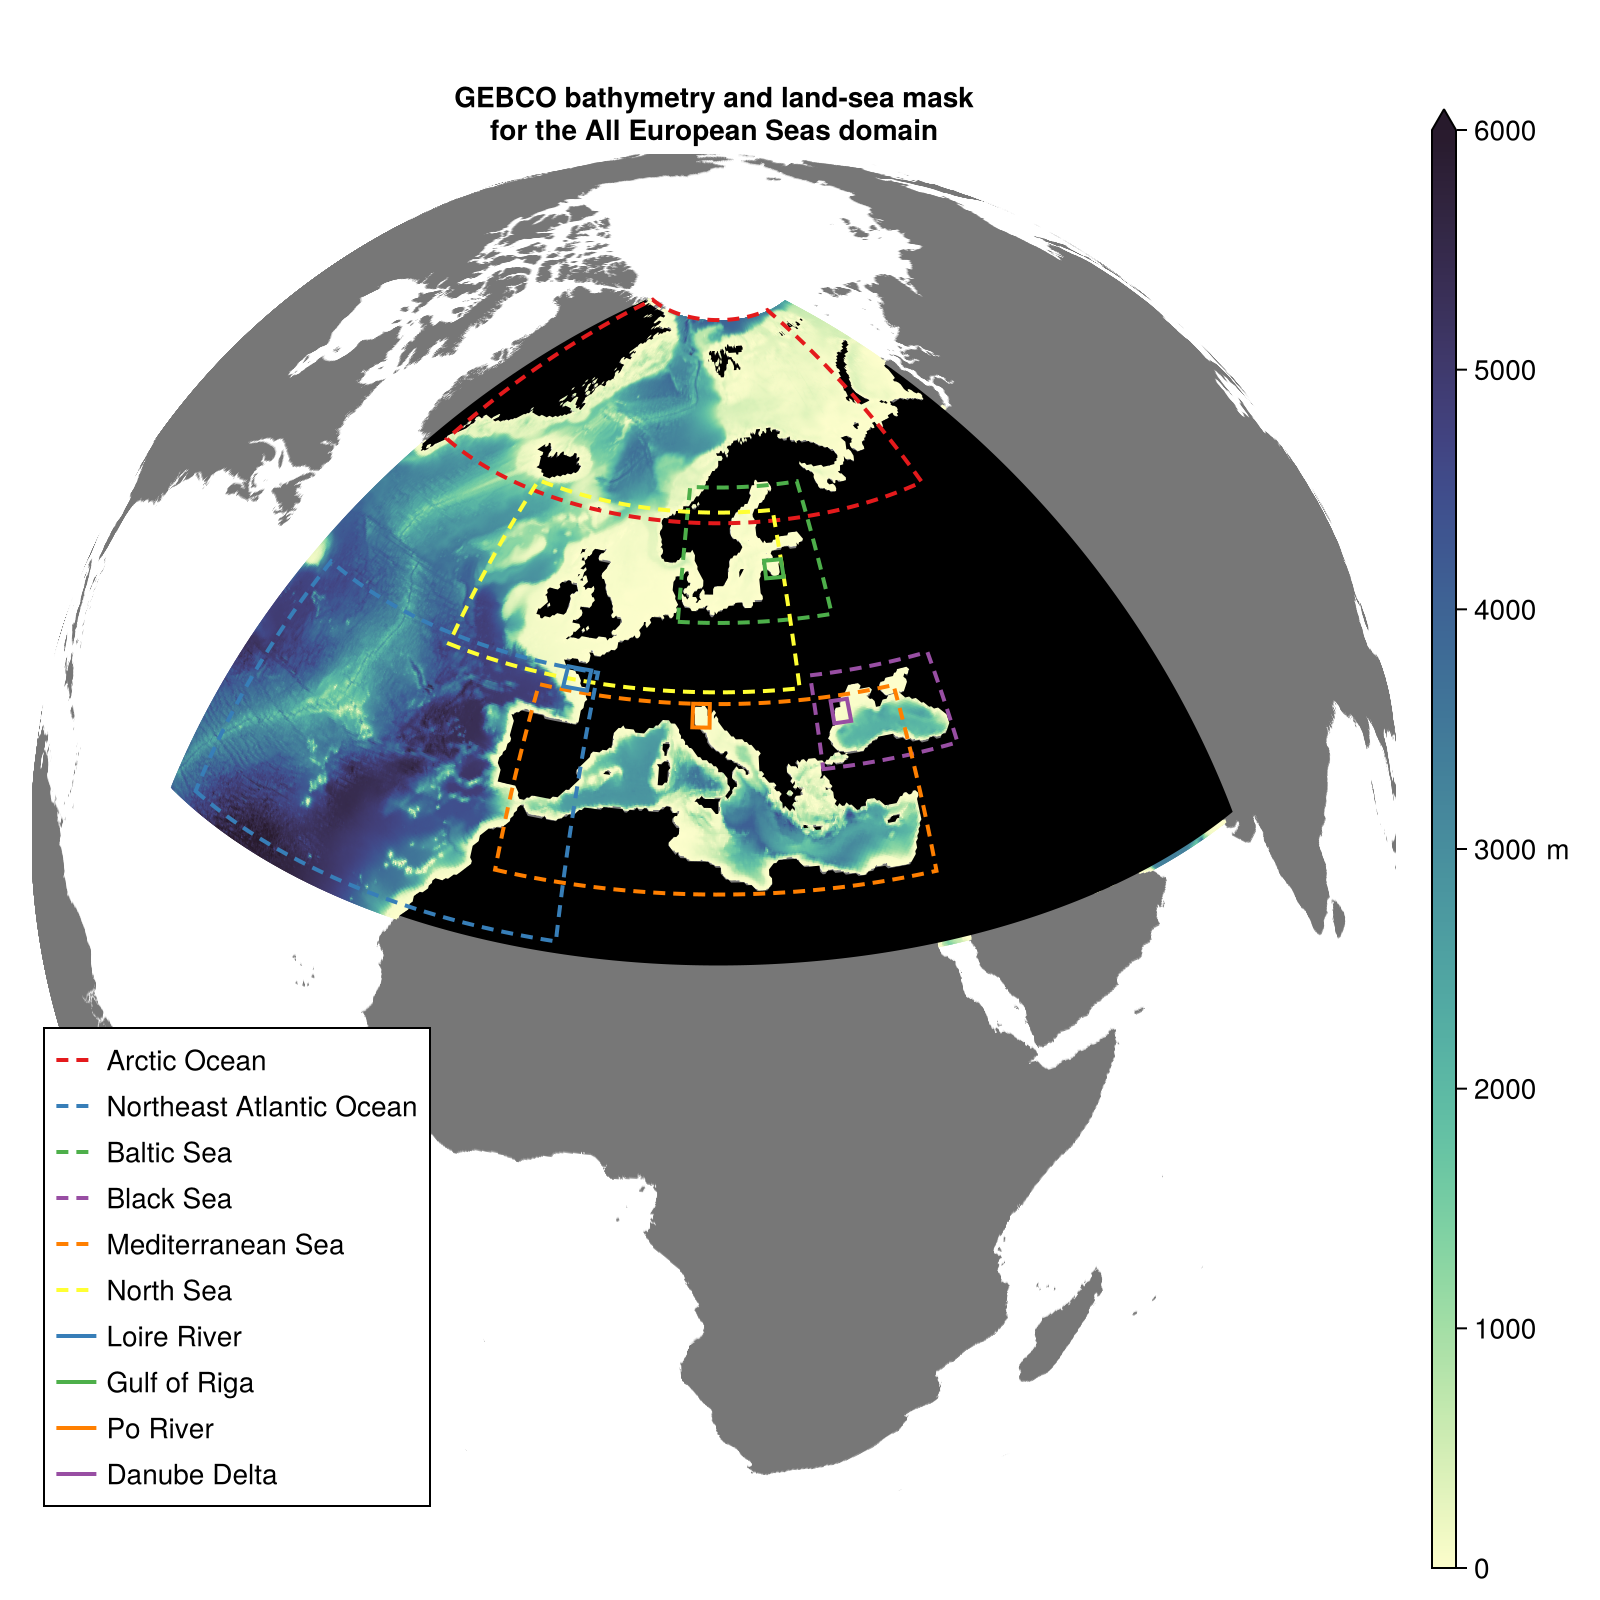
\includegraphics[width=12cm]{gebco_bathy_mask_domains3}
\caption{Regional domains (colored lines) for the gridded products overlaid on the GEBCO bathymetry and the surface land-sea mask, used to delimit the region where the interpolation is performed.\label{fig:gebco_bathy_mask_domains3}}
\end{figure*}

Along with the regional seas, 4~coastal regions have been defined. They are used for the creation of specific products near river mouths (see Section~\ref{sec:clim}) with a finer spatial resolution. Therefore, there is a total of 11~spatial regions where climatologies are created.

\begin{table*}[h!]
\caption{Spatial extend of the regional seas and the coastal areas.\label{tab:regions}}
\begin{tabular}{lrrrrll}
\tophline
Region	 					& West		& East		& South 		& North 		& Number of profiles	& Number of time series\\ 
\middlehline	
Arctic Sea 					& 45°W 		& 70°E		& 62°N		& 83°N		& 145417		& 0		\\
Baltic Sea					& 9.4°E		& 30.9°E		& 53°N		& 66°N		& 211608		& 98		\\
Black Sea					& 26.5°E 	& 42°E		& 40°N		& 48°N	 	& 75730		& 0		\\
Mediterranean Sea			& 6°W		& 36.375°E	& 30°N		& 46.375°N	& 253282		& 0		\\
North-East Atlantic Ocean 	& 42°W		& 0° 		& 24°N		& 48°N		& 389738		& 559	\\
North Sea 					& 5.4°W 		& 13°E		& 48°N		& 62°N		& 30804		& 134	\\
% Caribbean Sea				&          	& 			& 			& 			& 2863		& 91		\\
\middlehline	
Danube delta				& 28.5°E		& 30.5°E		& 43.7°N 	& 45.6°N		&			& \\
Gulf of Riga 				& 22.3°E 	& 25.0°E 	& 56.8°N 	& 58.4°N		&			& \\
Loire estuary				& 4°W		& 1°W 		& 6.25°N		& 48°N		&			& \\
Po river					 & 12°E		& 14.0°E		& 44°N		& 46.0°N		&			& \\
\bottomhline
\end{tabular}
\end{table*}

\subsection{Metadata\label{sec:metadata}}

Each observation comes with a \textit{Common Data Index} \citep[CDI,][]{Schaap2021,Schaap2022}, which provides details about the availability and geographical spreading of marine data sets managed by the SeaDataNet data centres. The index is based upon ISO~19115 and ISO~19139 standards, which define metadata for the description of geographic information, and supported by SeaDataNet Common Vocabularies (\url{https://vocab.seadatanet.org/search}). The CDI has been published in the Ocean Data Standards, managed by the Intergovernmental Oceanographic Commission of the UNESCO \citet{Schaap2021}.

Another relevant metadata field is the European Directory of Marine Organisations (EDMO) code, which indicates up-to-date addresses and activity profiles of the institution (research centers, universities, data center, \ldots) involved in the data holding. 

For each observation, the EDMO code and the CDI are concatenated to form a new variable called \textit{obsids}. This variable is then passed to the final netCDF product, ensuring that the information regarding the data originators is preverved and that their effort is correctly acknowledged in the final products. 

\subsection{Quality assessment\label{sec:dataqualitycontrol}}

One of the main added value of the aggregated datasets is the validation procedure applied to assess the quality of the measurements \citep{Barth2015,Lipizer2021,Lipizer2023}. The EMODnet Chemistry quality control chain involves the following steps:
\begin{enumerate}
\item Metadata completeness: it ensures that temporal and spatial information (longitude, latitude, sampling depth, station bottom depth, time) is present.
\item Harmonization of units and parameter names: it ensures that a given variable is always expressed with the same units and has always the same name (Tab.~\ref{tab:variables}). 
\item Quality flagging of data and metadata: a quality flag is assigned to the measurements and to their corresponding metadata.
\end{enumerate} 
The last step is described in details in \citet{Lipizer2023}, where the quality flag setting is explained. A particular attention is paid to the range check: each regional sea is decomposed into sub-domains and the range of acceptable values, for each variable, is set in those sub-domains. For instance, the acceptable chlorophyll concentration values in the Northern Adriatic Sea (strongly influenced by river discharge) are between 0 and 20~\unit{mg/m{^3}}, while this range is narrower in other sub-regions.

\subsection{Spatial distribution}

As stated in Section~\ref{sec:insitu}, the datasets are characterised by their strong heterogeneity. Figure~\ref{fig:phosphatedata} illustrates this features by displaying the phosphate and the ammonium data points, in the 6~regional domains from Tab.~\ref{tab:regions}. The differences between the spatial distributions of the two variables is obvious, with the ammonium mostly sampled in coastal areas, whereas the phosphate observations have a more extended spatial coverage.

\begin{figure*}[t]
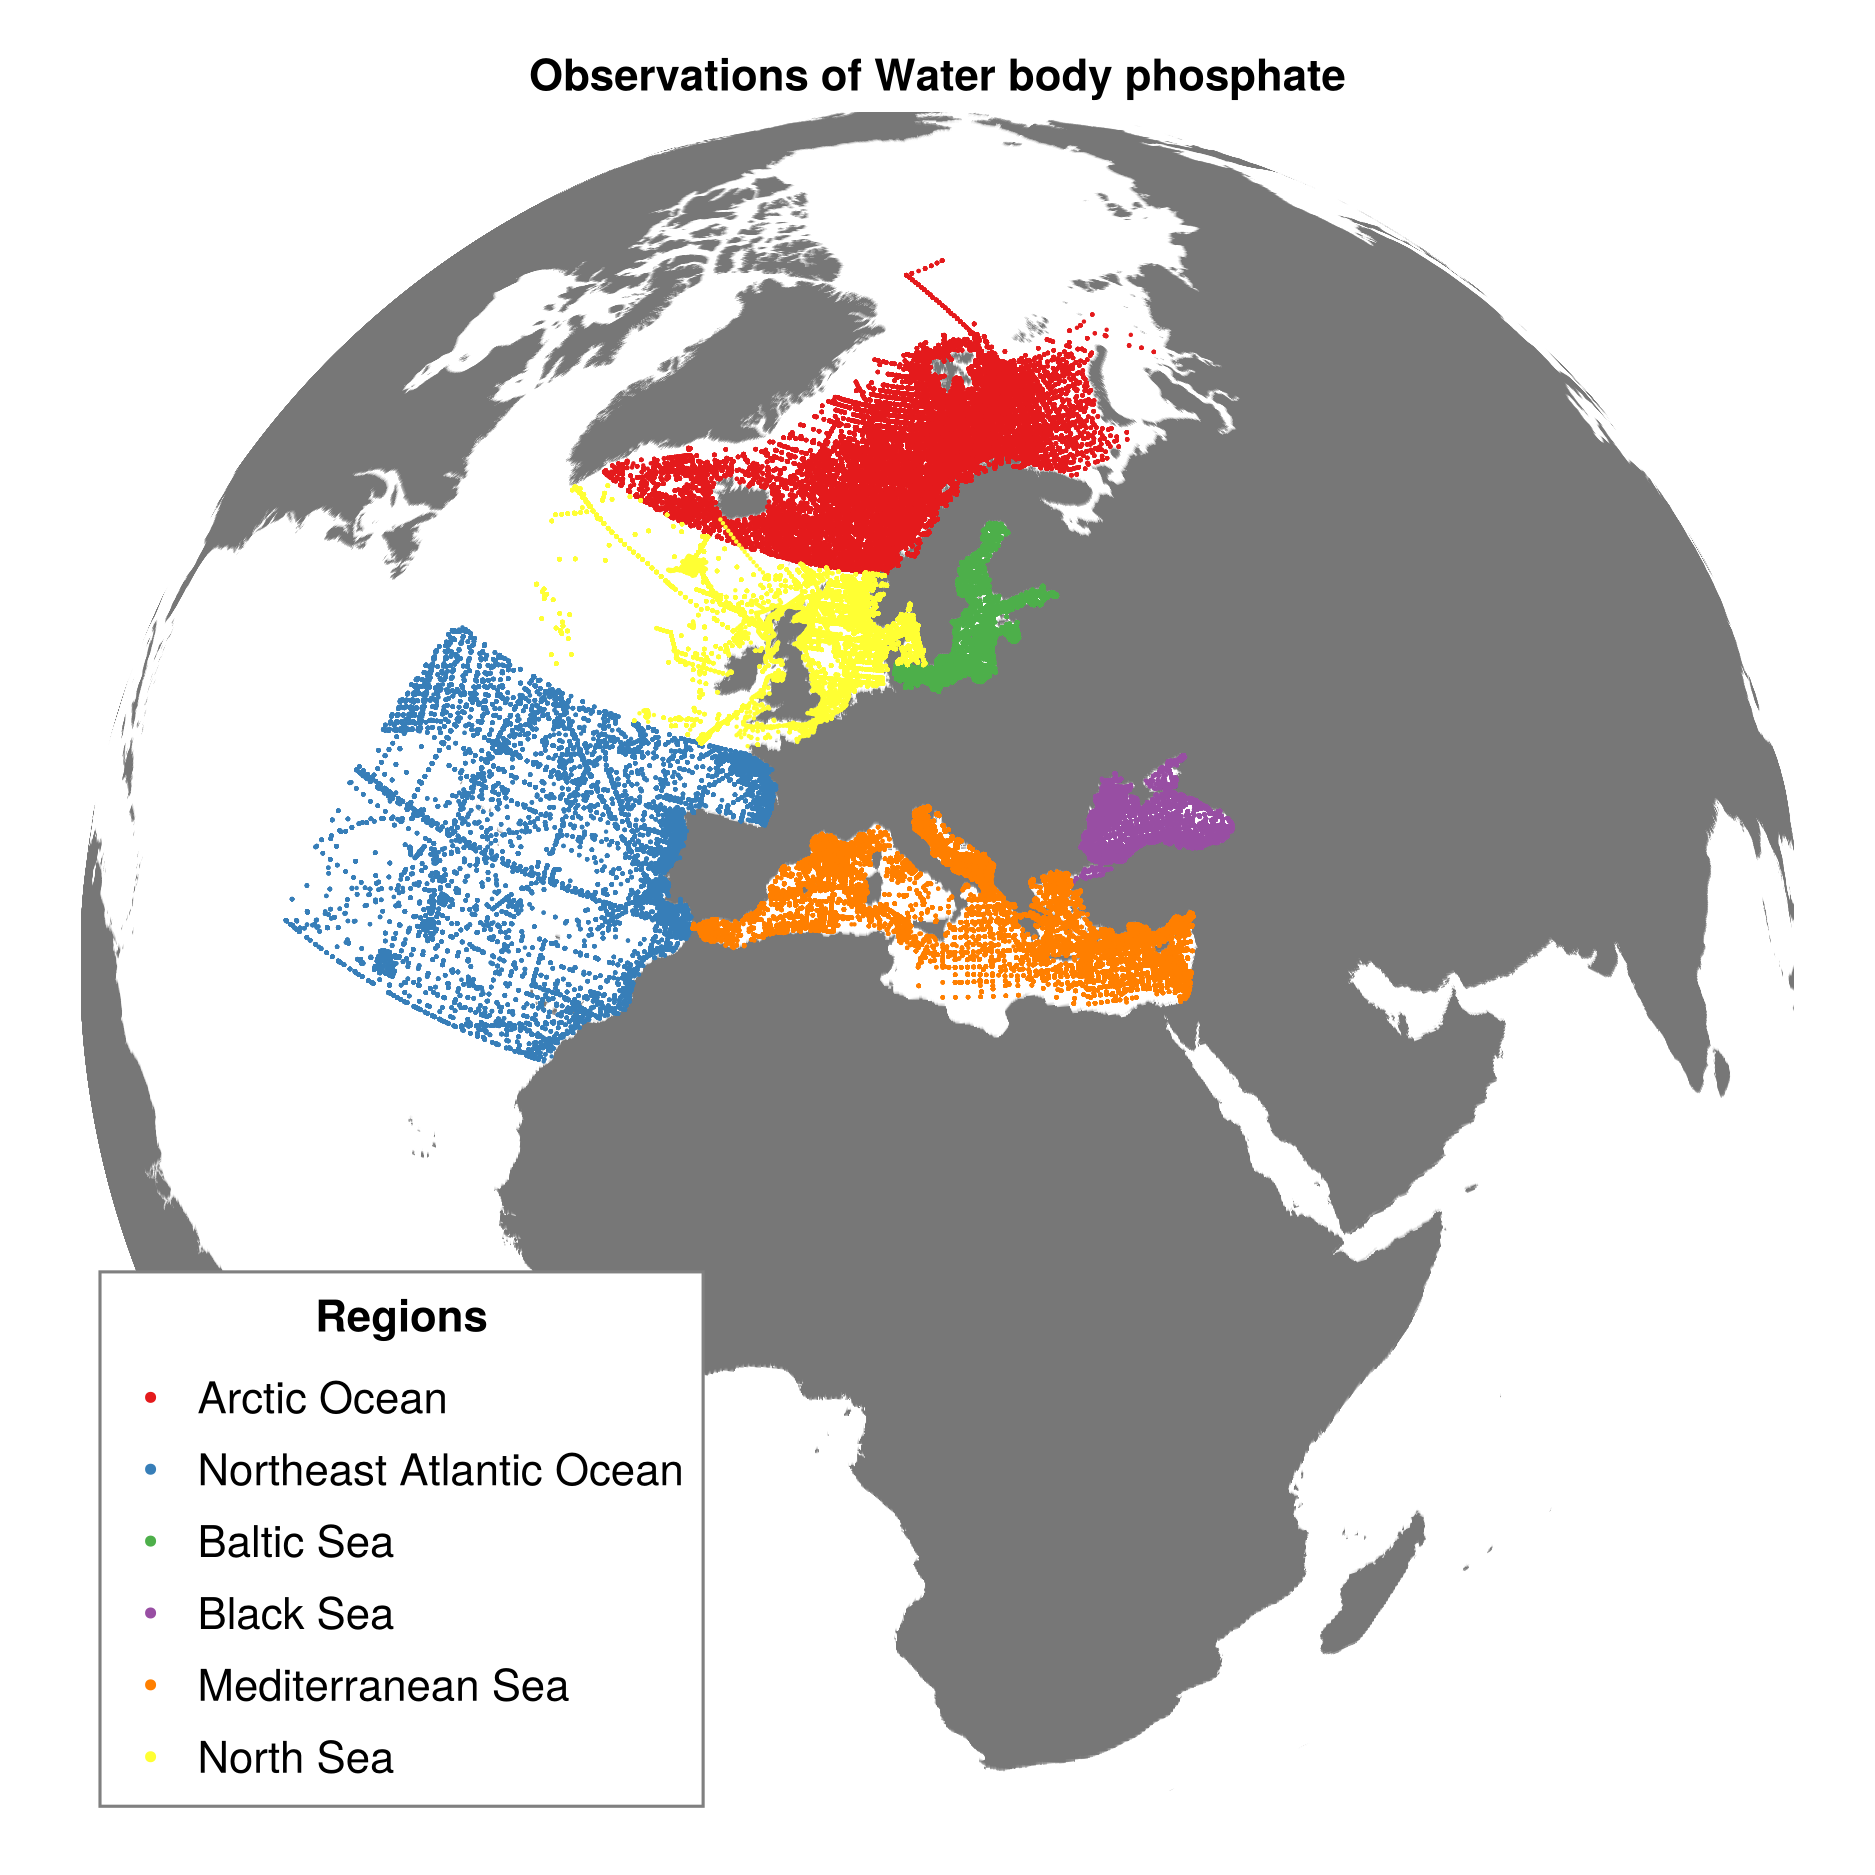
\includegraphics[width=.49\textwidth]{observations_Water_body_phosphate.png}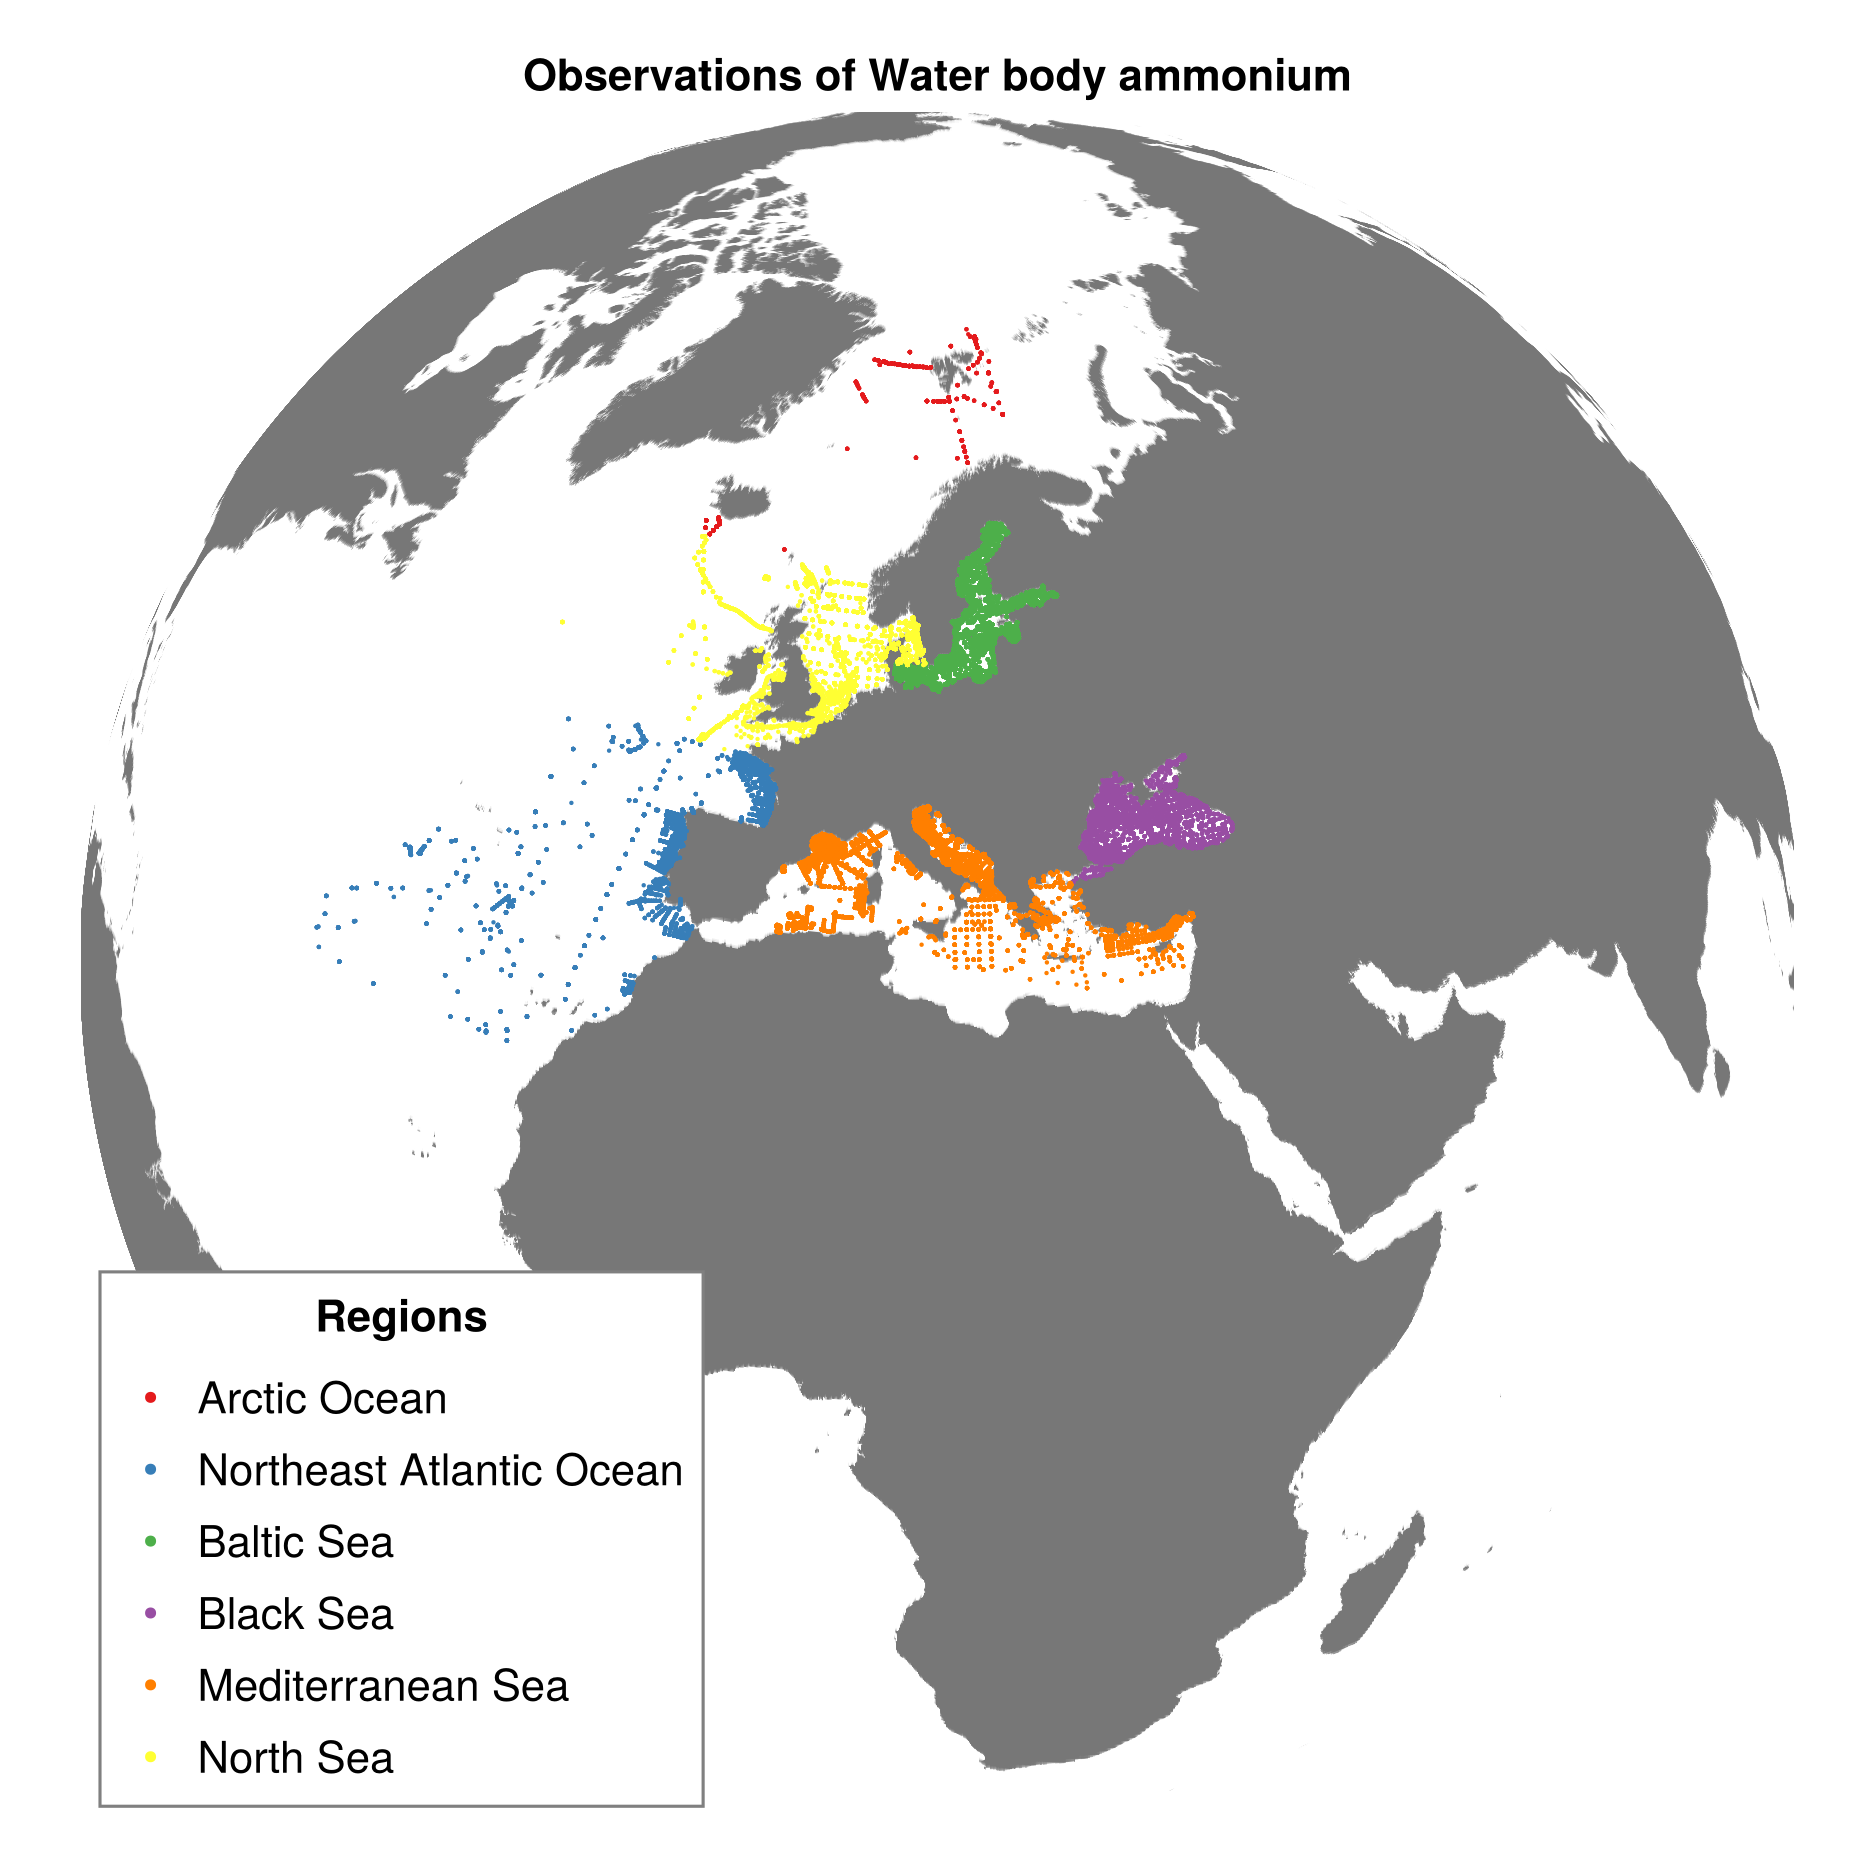
\includegraphics[width=.49\textwidth]{observations_Water_body_ammonium.png}
\caption{Locations of the phosphate concentration and the dissolved inorganic nitrogen concentration profiles.\label{fig:phosphatedata}}
\end{figure*}

The hexagonal binning (hexbin) plot (Fig.~\ref{fig:phosphatedatahexbin}) displays the number of observations within hexagonal cells. The regions with the highest coverage are located in the Baltic Sea and in the southern part of the North Sea, while in general lower data densities are found at the edges of the global domain. The Mediterranean sea also exhibits an inhomogeneous data coverage; with zones with almost no measurements at all (coastal zones of Tunisia and Lybia). The data coverage will obviously impact the quality of the gridded fields (Section~\ref{sec:clim}).

\begin{figure}[t]
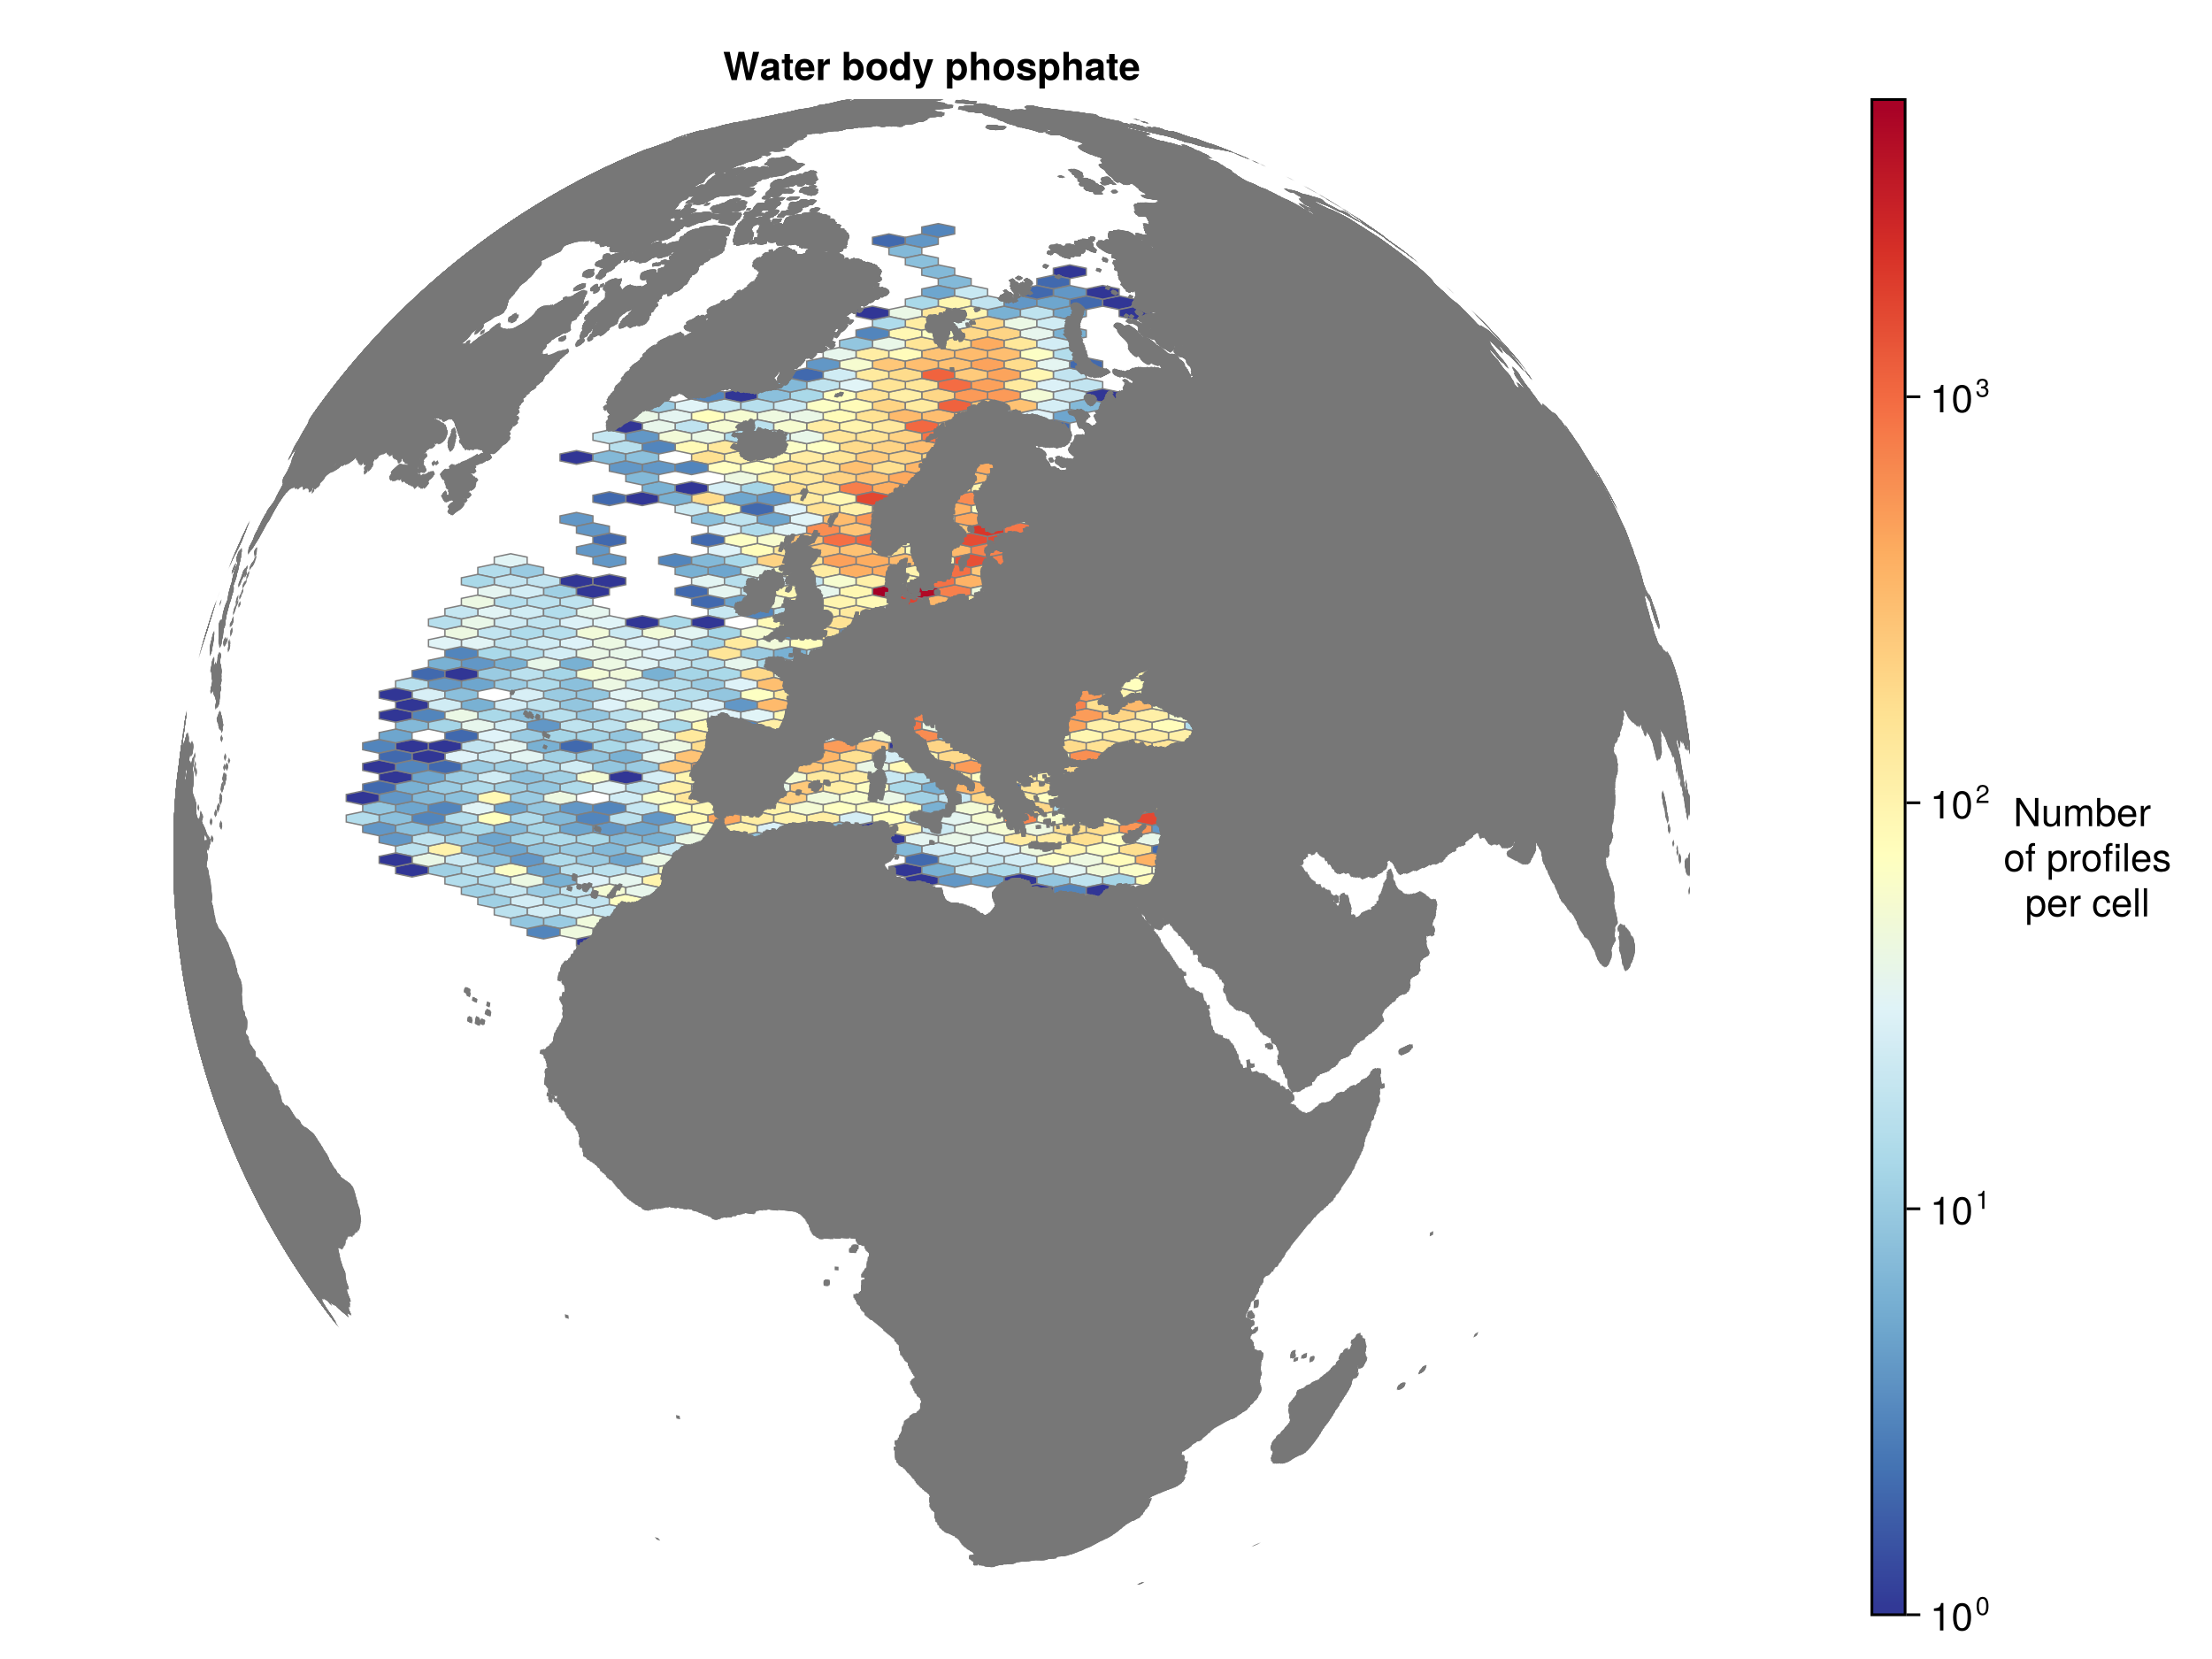
\includegraphics[width=8.3cm]{observations_Water_body_phosphate_hex.png}
\caption{Hexbin plot corresponding to the phosphate concentration profiles.\label{fig:phosphatedatahexbin}}
\end{figure}

\subsection{Temporal distribution}

The number of phosphate concentration observations per year and per months are shown in Fig.~\ref{fig:phosphatetime}. The first subplot exhibits an overall positive trend from 1960 oto 1990 approximately, followed by a more stationnary period. The last years have less observations, due to the typical time lag between the data collection and their inclusion into the international databases. Another striking feature visible in the histogram is the contributions by the different regions. For instance, the phosphate concentration in the North Sea only appear in the mid 1990's. The Baltic sea stands out as the largest contributor for this variable, despite its reduced geographical extension.

The second subplot shows the seasonal, with a factor 2 between the number of available of observations in the most sampled month (May) and in the least sample month (December). 

The histograms for the other variables are not included in the paper, but they also display similar heterogeneities in the temporal distribution, along with variations related to the variables themselves. 

\begin{figure*}[t]
\centering
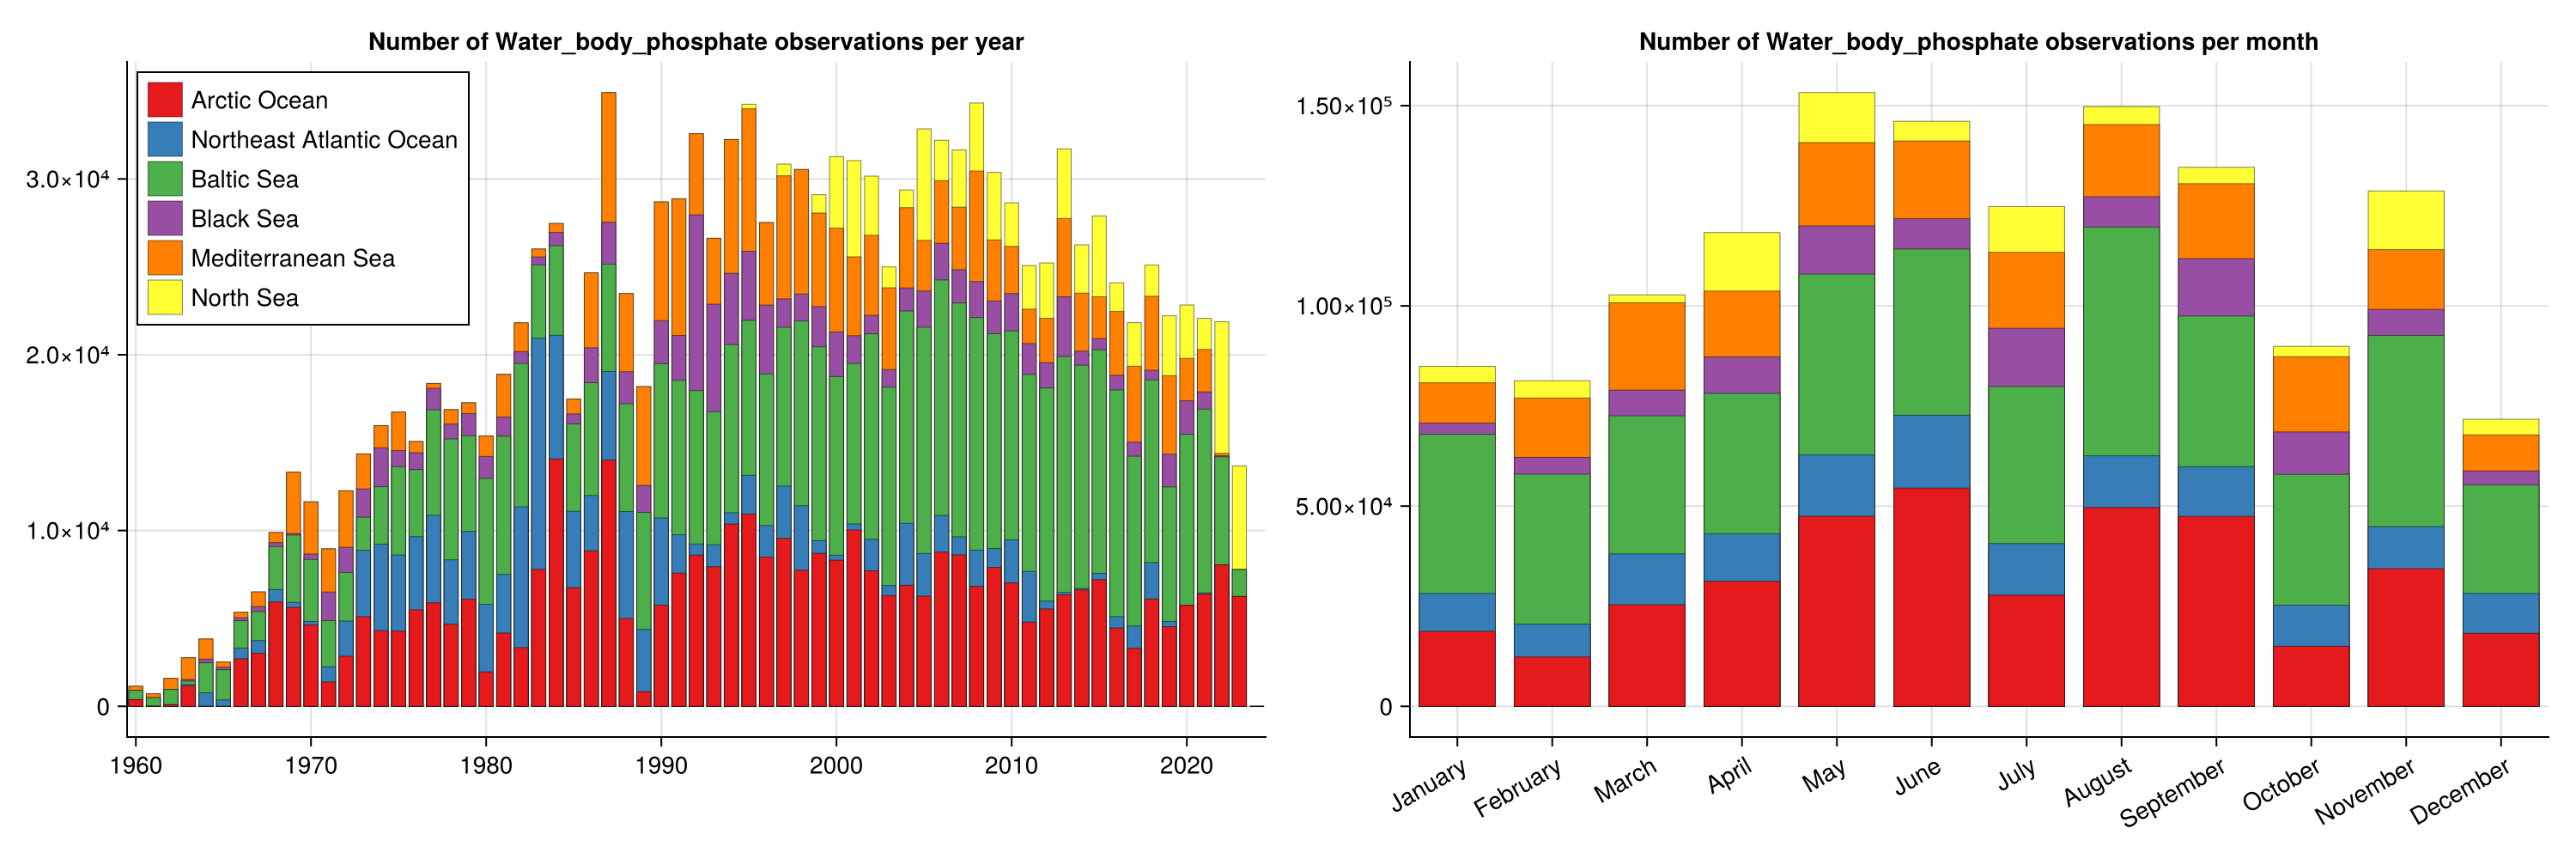
\includegraphics[width=\textwidth]{stacked_histogram_Water_body_phosphate.png}
\caption{Locations of the phosphate concentration profiles.\label{fig:phosphatetime}}
\end{figure*}


\subsection{Value distributions}

The histogram based on the observation values (Fig.~\ref{fig:histogram_value_Water_body_phosphate}) shows different patterns according to the variable considered. Most of the variables exhibit a distribution characterised by a dominant number of measurements for small concentrations (close to zero), and fewer observations of higher concentration. It is relevant to note that the distributions vary from one region to another, as depicted by the different colors in the histogram, see for instance the Arctic Ocean.

\begin{figure}[t]
\centering
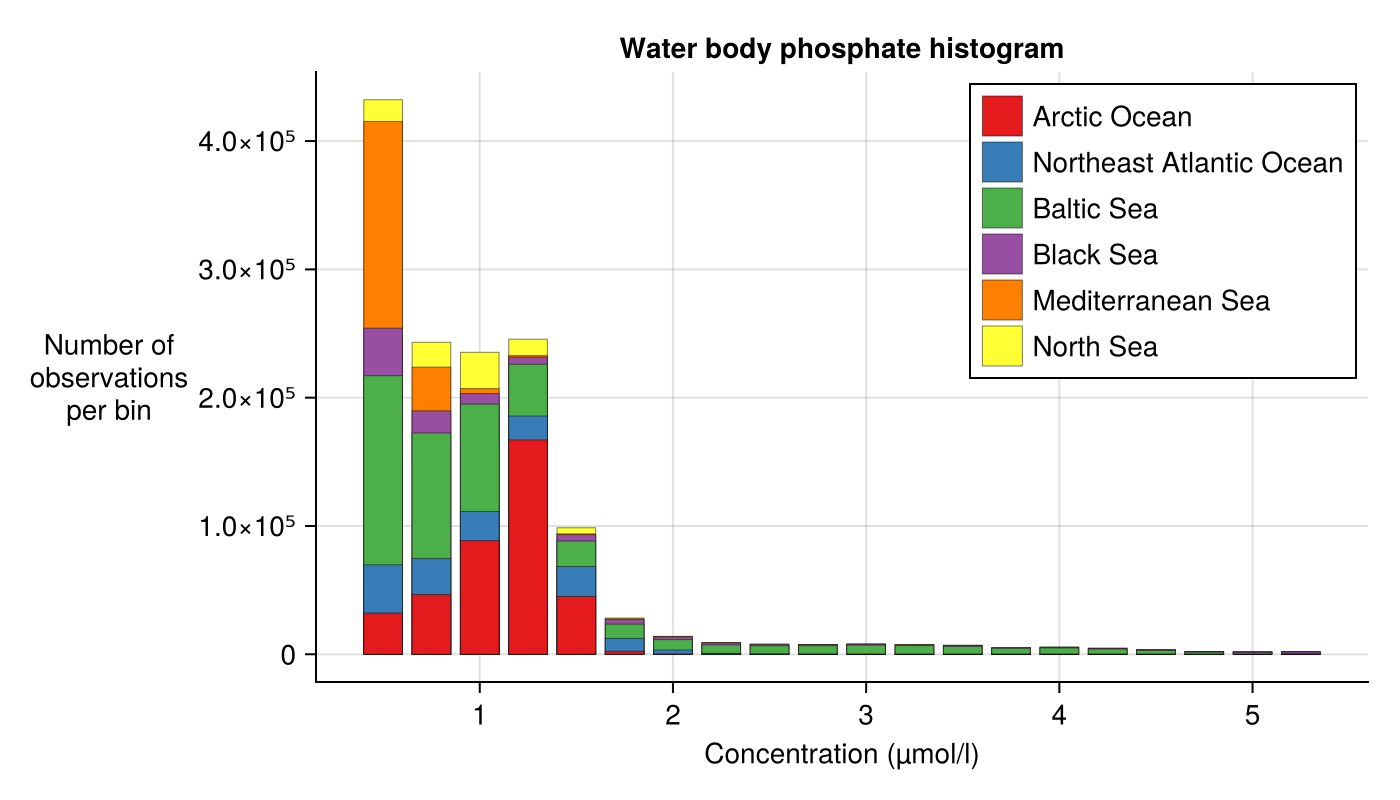
\includegraphics[width=.5\textwidth]{histogram_value_Water_body_phosphate.png}
\caption{Histogram corresponding to the phosphate concentration osbervations.\label{fig:histogram_value_Water_body_phosphate}}
\end{figure}


\subsection{File format}

The original data collections are provided as ODV (Ocean Data View) data collections, which is one of the standard format promoted by SeaDataNet marine data infrastructure \citep{Lowry2023}. Such collections are easily read then exported to another format using the ODV software tool \citep{SCHLITZER2002}. In the present work we exported the collections to netCDF files, which are in turn are used as input files for the preparation of the climatologies (next Section). Along with the data (coordinates, time, depth and observed values), a set of metadata is assigned to each measurement. Among them we find information about the instrument, the cruise and the institute that performed the measurements. 

\section{The gridding method\label{sec:method}}
%---------------------------------

In this paper, we refer to \textit{gridding} as the process of computing the values of a variable (for instance: sea water temperature) on the nodes of a regular grid, based on observations of that variable at different locations and times. The creation of gridded fields using sparse, in situ observations can be performed using different techniques. For the sake of simplicity, we will not review all of them but will insist on the distinction between two groups of techniques:
\begin{enumerate}
\item The interpolation techniques: the field has to contain (or pass through) all the data points. For two-dimensional cases, an example of such a method is the bi-linear interpolation. Due to the different types of noise affecting the measurements in the ocean (instrumental, representativeness, \ldots), such techniques are not the most suitable.
\item The approximation, also called analysis, where the field does not have to contain all the data points. Such category of technique is often preferred when it comes to process environmental data.
\end{enumerate}

Note that throughout this paper, we will use the terms "interpolation" and "analysis" to refer to the gridded technique, even if the method is not a strict interpolation.

The climatologies, consisting of a set of gridded fields for different depths and time periods, are produced by applying the Data Interpolating Variational Analysis in n dimensions (DIVAnd, see next Section) to the datasets presented in Section~\ref{sec:insitu}. Such gridded fields are frequently used in oceanography, for different purposes ranging from data visualisation to model initialisation or validation of measurements.  

Temperature and salinity (T and S) climatologies have been produced for various regions of the World Ocean using different interpolation techniques, yet climatologies for eutrophication-related variables are less frequent. The World Ocean Atlas (WOA) makes climatologies available for oxygen \citep[Dissolved Oxygen, Apparent Oxygen Utilization, and Oxygen Saturation,][]{Garcia2024} and for dissolved inorganic nutrients \citep[phosphate, nitrate and nitrate + nitrite, silicate,][]{Garcia2024b} at a resolution of 1°by 1° for the global ocean. The availability of measurements from the EMODnet Chemistry data collections makes it possible to increase the spatial resolution in certain domains, hence the interest of the regional products presented in this paper.


\subsection{DIVAnd\label{sec:divandmethod}}

The Data-Interpolating Variational Analysis in n dimensions method \citep[DIVAnd][]{BARTH2014} is designed to grid arbitrarily located observations in two or more dimensions, onto a curvilinear grid. Typically the dimensions are the longitude, the latitude, the depth and the time of the observations. DIVAnd in an evolution of the DIVA tool \citep{TROUPIN2012,BECKERS2014}, which was limited to 2-dimensional interpolations (hence climatologies were build by stacking 2D layers at different depths and for different periods). 

Mathematically, the DIVAnd technique is based on the minimisation of a cost function, in which the deviation from the observations, the deviation from a first guess (also called background or reference field) and abruptly varying fields are taken into account. The main strengths of the method with respect to widely used methods such as the Optimal Interpolation \citep[OI,][]{GANDIN1966,BRETHERTON1976} are its capacity to deal with very large datasets, as the numerical cost is almost independent from the number of observations, and the natural decoupling of regions based the topography. In other words, a basin separated from another by land is not affected by the observations located in the other basin.

The source code is written in Julia \citep{Bezanson2017}, a fast, dynamically-type programming language, designed to ensure high-performance computation. Julia ensures that high-resolution analysis using several millions of data points could be run in reasonable times, i.e. maximum a few days for the largest domain. This is necessary as usually to create a regional climatology, it is necessary to repeat the analysis several times in order to adapt the parameters and possibly remove suspect observations.

DIVAnd has already been applied applied on a wide range of ocean variables such as temperature, salinity \citep{COATANOAN2021}, sea surface height \citep{DOGLIONI2023}, velocity \citep{TROUPIN2022}, dissolved inorganic nutrients \citep{BELGACEM2021} or oxygen concentration \citep{CLIMATO2023}. In this work, the version v2.7.12 of the code \citep{BARTH2024DIVAnd} is used.

\subsection{Implementation}

For the creation of the gridded maps, the regional groups are provided with a set of Jupyter notebooks \citep[https://jupyter.org][]{KLUYVER2016}, which serve as guidelines explaining all the steps to perform for the creation of a climatology:
\begin{enumerate}
\item Data reading and file format conversion;
\item Creation of the land-sea mask based on the bathymetry;
\item Parameter optimisation;
\item Analysis;
\item Creation of figures;
\item Creation of metadata for the inclusion in catalogue.
\end{enumerate}
The relevant notebooks (those dealing with the analysis) are then modified according to the specificities of each domain. They have been submitted for publication \citep{TROUPIN2025}.

The GEBCO bathymetry \citep[2021 grid,][]{GEBCO2021} was used with a resolution reduced by a factor 4 with respect to the original, was used for the creation of the land-sea mask
needed by DIVAnd (Fig.~\ref{fig:gebco_bathy_mask_domains3}). The role of the land-sea mask is to delimit the region where the interpolation is performed, since the cost function (see previous Section) is only computer over cells corresponding to the sea. 

For the sake of conciseness, the rest of the maunscript will focus on the "All European Seas" products. The procedure applied for the creation of the other climatologies is similar, and details can be found in the technical report by \citep{BUGA2021}.

\subsection{Analysis parameters}

A brief description of the main analysis parameters is useful to understand how the products are generated.

\subsubsection{The correlation lengths}

This parameter defines the spatial or temporal scales  over which observations are correlated. In general, for a climatology, this parameter can have up to 4 components: longitude, latitude and depth. Usually the meridional and zonal components are assigned the same value (horizontal isotropy). The vertical correlation length can also be varying vertically and horizontally. For the products presented in this paper, no temporal correlation length was used, i.e. the time periods (months or seasons) are assumed to be uncorrelated. 

For the All European Seas, the horizontal correlation length was set to vary from region to region, with the following strategy: each sub-region is assigned a correlation length; to ensure a smooth transition between those sub-regions, a diffusion filter is applied. Finally, the correlation length is decrease toward the coast, leading to the spatial structure shown in Fig.~\ref{fig:correlation_length}(a). The vertical correlation is increased with depth in order to represent the stronger stratification existing at the surface (Fig.~\ref{fig:correlation_length}(b)).

The netCDF file storing the correlation length on the analysis grid is provided in the Addition Material section.

\begin{figure*}[t]
\centering
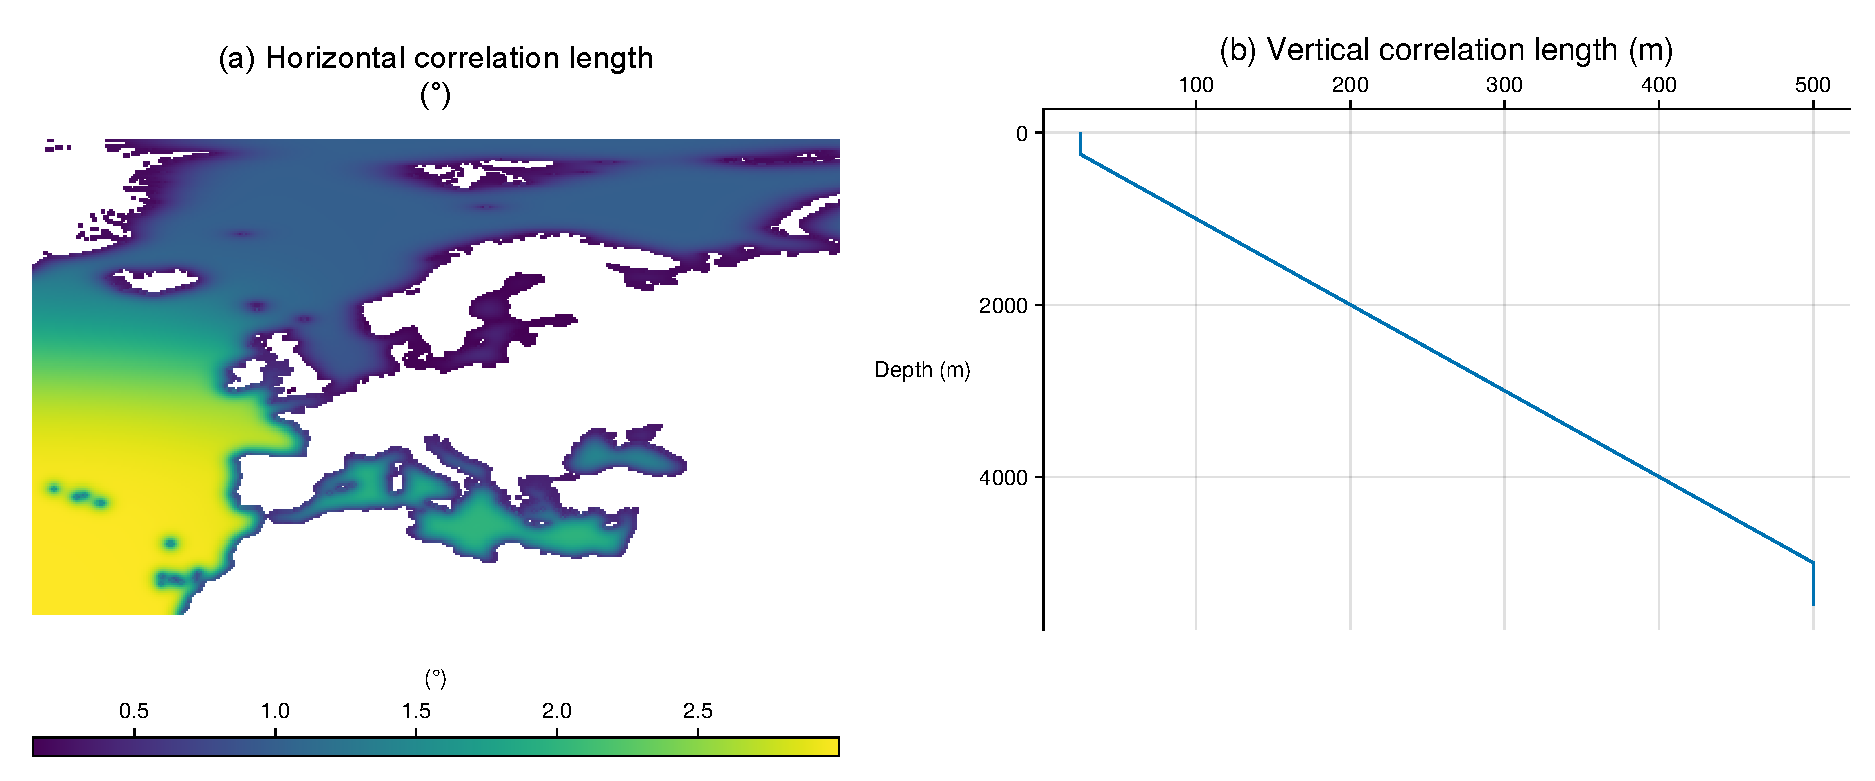
\includegraphics[width=\textwidth]{correlation_length.pdf}
\caption{Correlation lengths for the All European Seas: (a) horizontal and (b) vertical.\label{fig:correlation_length}}
\end{figure*}

\subsubsection{Signal-to-noise ratio}

This parameter is defined as the error variance of the observations normalized by the error variance of the background field. It can be a scalar (all observations have the same error variance and their errors are decorrelated), a vector (all observations can have a different error variance and their errors are decorrelated) or a matrix (all observations can have a different error variance and their errors can be correlated). 

A large value of the noise-to-signal ratio has the effect of smoothing the resulting analysis, removing the spatial variability. For the All European Seas product, the overal noise-to-signal ratio was set to 2.0. Then the weights, based on the distance between osbervations, were computed for every data points. The goal of this step is to decrease the weight of osbervations coming from a high-resolution instrument (for instance glider) or from time series with a high frequency of acquisition. The final noise-to-signal ratio is then a vector obtained by multiplying the initial value (2.0) with the weights.

\subsection{Background field}

The cost function implemented by DIVAnd considers the anomalies with respect to a background (also called reference) field. There are several ways to compute this background field, the most direct option is to take a spatially uniform field, for a given depth level, with the value equal to the mean of all the observations. The strategy adopted to compute the background field for all All European Seas product is to create a gridded field using all the available observations (whatever the month or year) and with the correlation length and the noise-to-signal ratio both multiplied by a factor 5. 

%----------------------------------------------
\section{Gridded climatologies\label{sec:clim}}
%----------------------------------------------

The URLs of the netCDF files storing the climatologies are provided at the end of the paper (Table~\ref{tab:doiProducts}).

\subsection{File preparation}

The original files storing the observations are provided as ODV collections \citep[Ocean Data View,][]{SCHLITZER2002}. There are then converted to ODV netCDF format, built upon the CF conventions, where the observations are organised by profiles as in the original collections. During this conversion, we ensure that the relevant metadata (i.e. those relative to the originators: EDMO codes and CDIs) are conserved in the exported files. Finally, for performance purposes, the ODV netCDF files are converted to ragged array netCDF, since the information about the profiles is not necessary any more for the interpolation. This final conversion is optional, but it offers the advantage of reducing the time needed to read the observations from the different regions is strongly reduced.

For instance, on a desktop machine, reading the phosphate observations from the ODV netCDF file for the North-East Atlantic Ocean takes close to 30 minutes. Using the ragged array netCDF, the executation takes 27~ms (averaging several tries). These conversion operations were performed with ODV version 5.7.2 \citep{Schlitzer2024}.

\subsection{Product types\label{sec:products}}

Three sets of climatologies were produced, grouped according to their spatial extent (detailed in Tab.~\ref{tab:regions}): 
\begin{enumerate}
\item The \textit{All European Seas} products: they consist of monthly fields (considering all the available data for the period 1960-2024), computed over a spatial domain covering all the regional seas.
\item The \textit{Sea Region} products: the are computed for seasons and for periods of 6 years, using a moving 6-year window. The definition of the seasons and the 6-year time periods are not the same for all the regions. 
\item The \textit{Coastal Area} products: they are computed over small areas near river mouth, and at seasonal scale. The spatial resolution is increased with respect to the Sea Region climatologies.
\end{enumerate}

\subsection{File format}

The output of the analysis is a set of netCDF files storing the gridded fields generated by the analysis are written in netCDF \citep{Rew1990,Brown1993,Rew2006}, making use of the NCDatasets.jl Julia library \citep{Barth2024}. The file sizes depend on the type of product (as defined in Section~\ref{sec:products}) and the region of interest. The largest files are for the North-east Atlantic region, approximately 10~\unit{GB}.

In order to reduce the file sizes (optional), advanced compression techniques \citep{Silver2017,Zender2016} can be applied through the use of the nco tool \citep[netCDF operators,][]{Zender2008}. One can expect a file size reduction by a factor of 3-10, depending on the algorithm and the original file.

\subsection{Gridded variables}

The main variable stores the 4-dimension gridded field (e.g., longitude, latitude, time and depth) for each of the 6 selected variables. In addition, a relative error field informs about the quality of the results. It typically exhibits larger values in regions with where no observations were collected, while the value are the lowest where the coverage is most dense. The term "relative" means that the error field is scaled by the background variance. The reason why the relative error (instead of the absolute error) is provided arises from the difficulty to compute the background variance.  

The error field is used to mask out the gridded field in regions where the error is considered to be too high. The decision to compute those masked fields comes from the discussion among the EMODnet-Chemistry experts, who recommended to only the display the gridded fields where (enough) observations are available. In practice, gridded fields masked using relative error threshold of 30\% and 50\% are calculated. The field masked with the 30\% error threshold is displayed as the principal layer in the Web Map Service (WMS). The motivation is to prevent users from interpreting the results where no background information exists. 

\begin{figure*}[t]
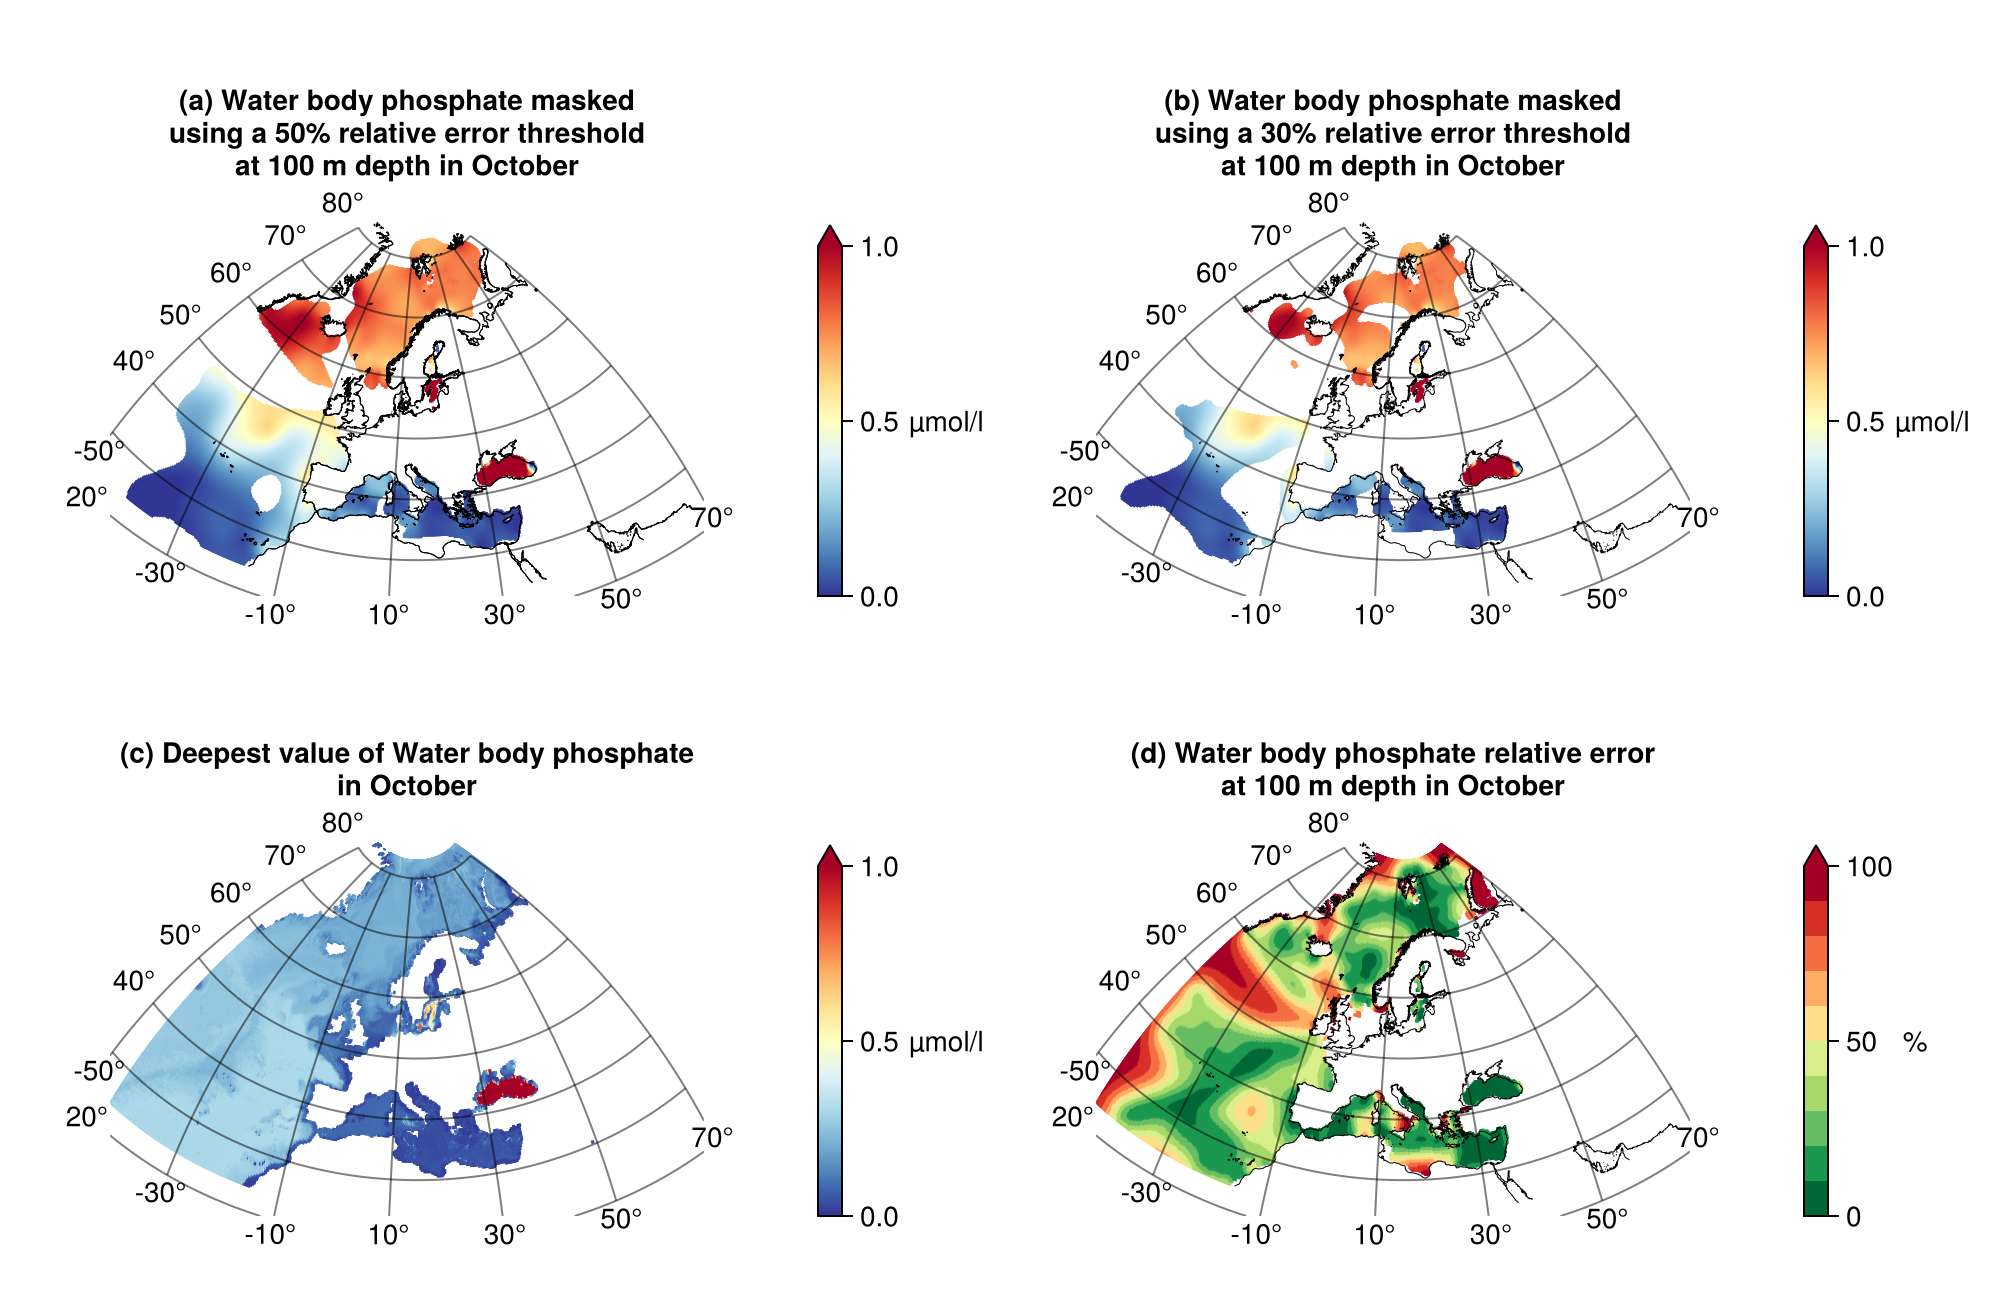
\includegraphics[width=\textwidth]{Water_body_phosphate_depth-100_month-10_additional_fields.png}
\caption{Additional fields computed along with the main analysis.\label{fig:additionalfields}}
\end{figure*}

Other variables containing the deepest values, masked with the same relative error thresholds, are also computed. These variables were also created following discussions with group of experts, thus underlying the user-driven developments of the code.

\subsection{Metadata and product publication}

Complete and standardised metadata are essential when it comes to share the data and data products with a wider audience, especially in the light of the FAIR principles. This is why the EMODnet Chemistry climatologies are filled with many pieces of information concerning the parameters (through parameter and search keywords), the dataset provenance, the creators of the product, links to the documentation etc. They are stored as global attributes in the netCDF files.

In addition, the \textit{obsid} variable, a vector of strings constructed using the EDMO code, for the identification of the institution, and the CDI for the identification of the observation (Section~\ref{sec:metadata}), is also written in the netCDF file, ensuring that every single observations can be traced back to its originator.

As all the EMODnet products, the climatologies have to be available through the EMODnet product catalog \citep[][https://emodnet.ec.europa.eu/en]{BEJA2024}

\subsection{Validation}

The quality and the validation of the final products rely on the assessment of the different steps of the processing:
\begin{enumerate}
\item The quality control of the aggregated datasets used as the input to the DIVAnd tool (Section~\ref{sec:dataqualitycontrol});
\item The overall capability of DIVAnd to generate interpolated fields consistent with the observations, as demonstrated in previously published literature (Section~\ref{sec:divandmethod});
\item The absence of unrealistic features (anomalous values, strong gradients, boundary problems, \ldots) in the gridded products.
\end{enumerate}

An additional, frequently performed step for the validation consists in comparing the results with an existing climatology. For our products, the most obvious candidate is the World Ocean Atlas, which provides climatologies for the oxygen concentration \citep{Garcia2024} and for dissolved inorganic nutrients \citep{Garcia2024b}. Since the EMODnet climatologies consist of regional gridded fields, they have the advantage to offer finer spatial resolutions than global products. Another advantage of the EMODnet products is the relative error field (see for instance Fig.~\ref{fig:additionalfields}) computed by DIVAnd. The WOA also provides the standard error of analysis, based on the differences between the objectively analyzed and statistical mean fields \citep{Levitus2012}.

The phosphate concentration fields from DIVAnd and from WOA are presented in Fig.~\ref{fig:comparisonWOA}. The goal of this comparison is not to perform a deep analysis of the differences, but rather to examine if the two fields are similar (range of the variables, main spatial features). One has to keep in mind that the input datasets for the two products are not exactly the same. 

\begin{figure*}[t]
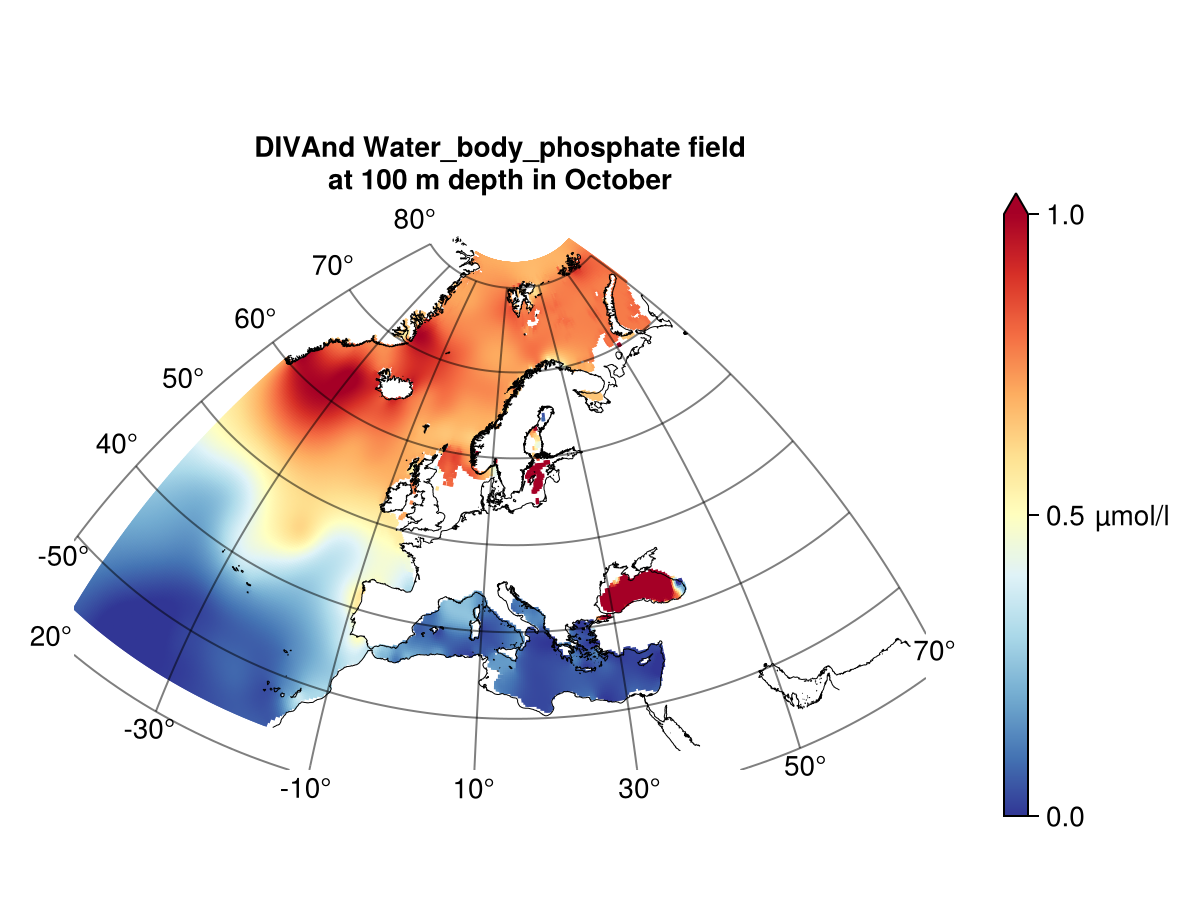
\includegraphics[width=.49\textwidth]{Water_body_phosphate_depth-100_month-10_DIVAnd}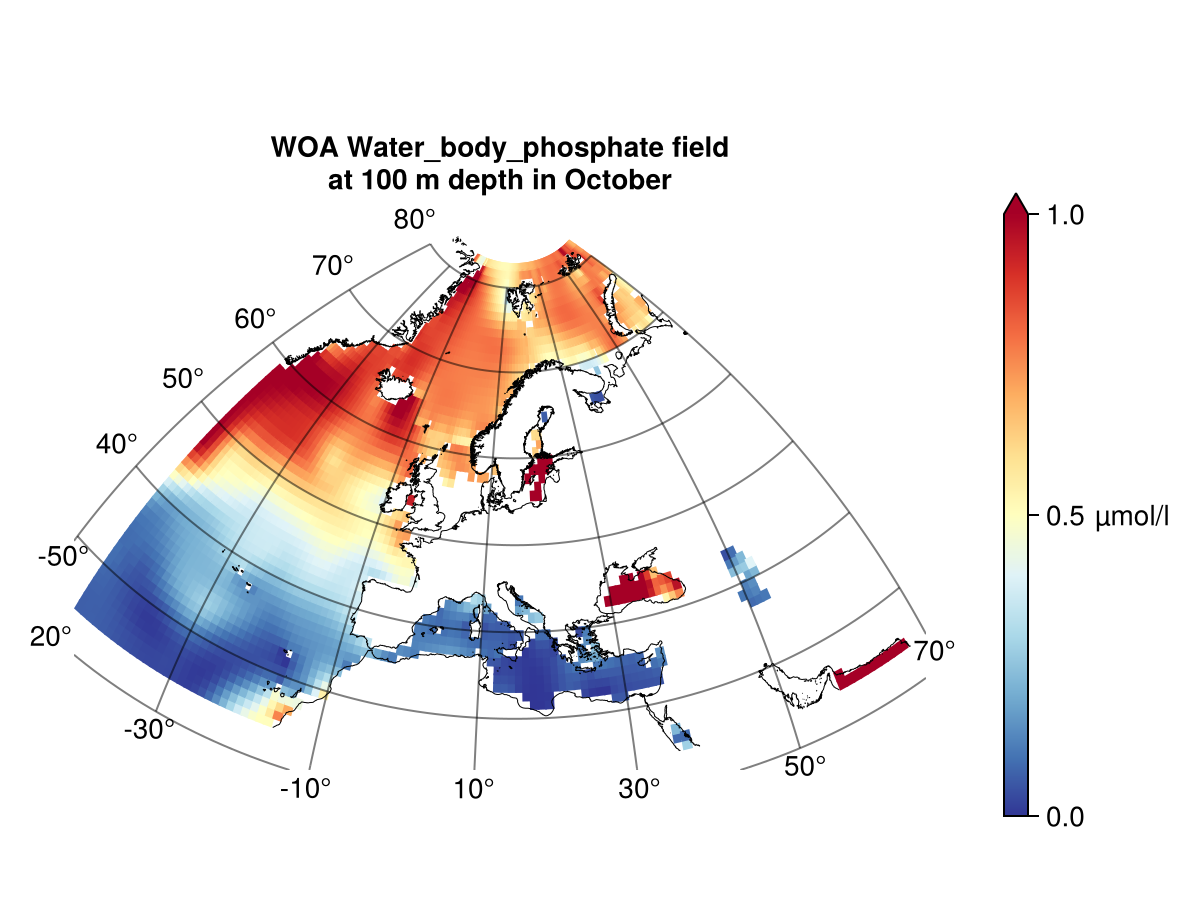
\includegraphics[width=.49\textwidth]{Water_body_phosphate_depth-100_month-10_WOA.png}
\caption{Analysis of phosphate concentration at 100 depth in October obtained with DIVAnd (left) and from World Ocean Atlas.\label{fig:comparisonWOA}}
\end{figure*}


\subsection{Result exploitation}

The climatologies can be exploited in various ways and by a diverse user group. The following descriptions is not meant to be exhaustive, it merely offers a few relevant applications.

\subsubsection{Visualisation}

Climatologies can be used to display ocean properties, for instance in a teaching context. While sea water temperature maps have made their way to mainstream media, thanks to marine heat waves, maps showing concentrations of oxygen or nutrients are rarely presented. Considering the example of Fig.~\ref{fig:additionalfields}, one can directly see the higher abundance of phosphate north of 60°N, the lower concentrations in the Mediterranean Sea contrasting with the larger values in the Black Sea.

Another aspect of the visualisation is related to the error fields: one can clearly see where the data gaps are located and possibly where the efforts should be directed to fill these gaps. This can be done either by increasing the sampling campaigns in those error or high relative error, or to increase the effort in terms of data rescue.

\subsubsection{Quality control of new observations}

They are several criteria to detect incorrect data, or to be more accurate, to assign a quality flag to measurements \citep{CUMMINGS2011,CABANES2021}. The most natural test consists of checking if the observed value falls inside a given range. For a given variable, such range can be global, i.e. the same for any region, any depth or any time period. A more elaborated criterion relies on a climatology: the comparison is performed with respect to the "normal" values (defined by the World Meteorological Organization as the 30-year average of data). If the difference between the newly acquired observation and the corresponding climatologies (called the residual) is larger than a select threshold (based on the standard deviation, for example), then that observations can be considered as suspect.

For the EMODnet-Chemistry climatologies, the residuals obtained from the pan-European gridded fields were provided to each regional leader. They were then asked to flag out suspect data, basing their decision on the values of the residuals. Finally, a new analysis was performed on a dataset in which the suspect observations were discarded. Figure~\ref{fig:residuals}) shows the phosphate residuals which have a value larger than 10~\unit{\mu~mol/l}. Those points are mostly distributed along the coast, which is where the variability is the strongest. 

A large value for the residual is not synonym of bad data point: the suspect observation has to be reported back to the corresponding regional leader, who will then contact the data provider before deciding if the measurement is correct or not. This process highlights the need to always keep the data provider in the loop, as they have the local expertise in terms of processes taking place in the region of interest, as well as the conditions during which the data acquisition was performed. 

\begin{figure}[t]
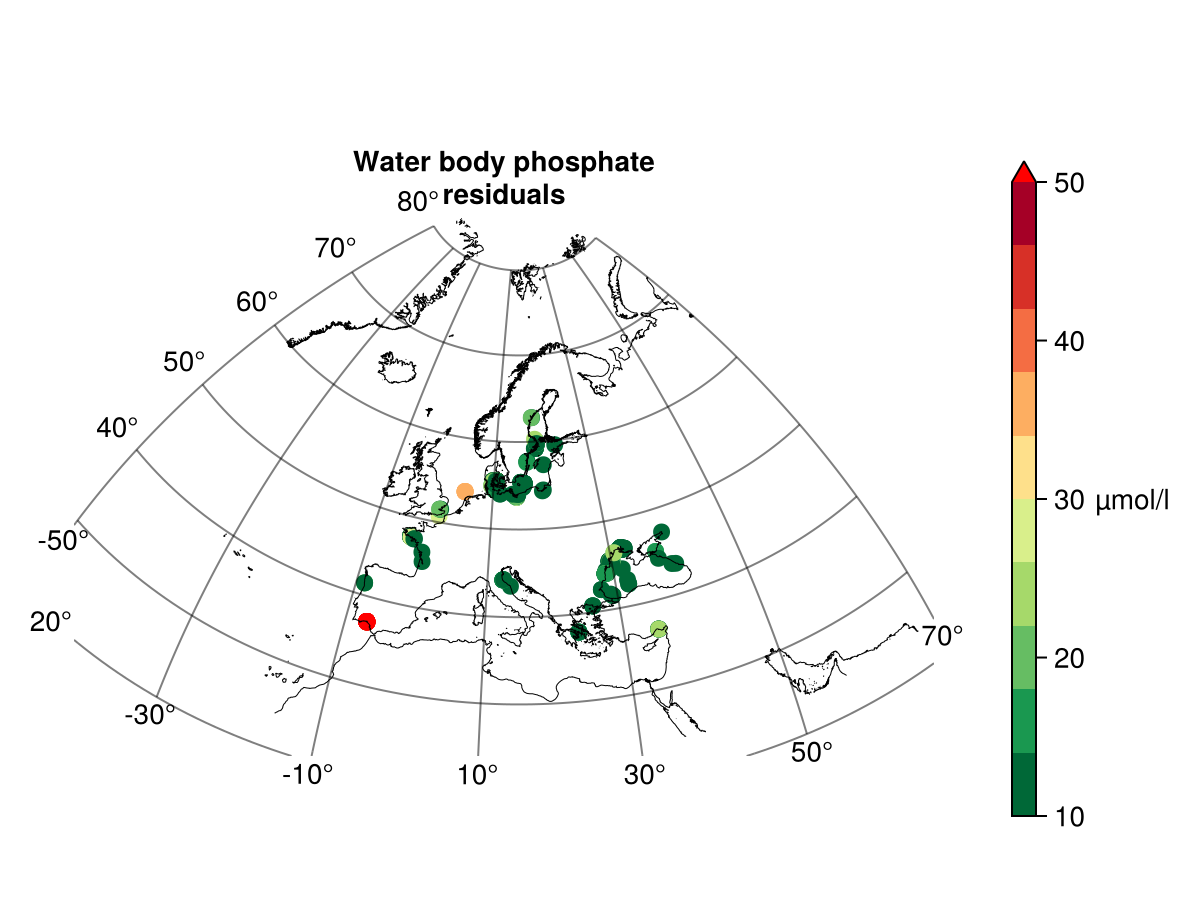
\includegraphics[width=8.3cm]{residuals_Water_body_phosphate.png}
\caption{Residuals (observations minus climatology) corresponding to phosphate concentration.\label{fig:residuals}}
\end{figure}

\subsubsection{Assessment of marine ecosystems}

Combining information about the nutrient and the oxygen in a given region allows one to evaluate the ecosystem health and examine its role in terms of primary production or carbon sequestration.

Concretely, since 2009, EMODnet Chemistry has interacted with the stakeholders involved in the Regional Seas Conventions (OSPAR, HELCOM, \ldots) and the Marine Strategy Framework Directive (MSFD). A Board of experts on the MSFD, formed in 2017, aims to advise the consortium on the products and services: parameters, spatial and temporal resolutions of the data products. Doing so, it is expected that the data collections and the climatologies will contribute to the MSFD Descriptors D5 (eutrophication), among others.

\conclusions  
This paper describes the creation of climatologies for eutrophication variables (ammonium, chlorophyll-a, dissolved inorganic nitrogen, dissolved oxygen, phosphate and silicate) in 11 regional domains. Three groups of regions are considered: All European Seas, Regional Seas and Coastal Zones. The climatologies are based on in situ measurements which underwent quality control. Those datasets are then fed as in input to the DIVAnd software tool. 

The products consist of netCDF files storing the gridded fields for the specified time periods and depth levels. They can be downloaded and reused for many purposed: visualisation, improved quality control, validation of new measurements, \ldots. 

Possible improvements rely on the increased availability of data, coming from the acquisition of new measurements, but also from initiatives such as EMODnet Data Ingestion \citep{IONA2024}. This initiative strives to reach out, motivate and support potential data providers, in order to make sure that the data they collected can make their way to centralised portal with standardised and complete metadata, hence strengthening the "Collect once, use many times" mentioned in the introduction. 

The interpolation technique can also be improved, for instance by allowing the interpolation along isopycnal, rather than at fixed depths. This would reduce the mixing effects and allow for a better representation of the water masses. Most of the recent developments of DIVAnd are driven by issues or suggestions raised by the user community, and the future developments will continue to follow that principle. Finally, a fundamental aspect of the climatology preparation is to make sure that any external user can take an existing piece of code (Julia script or Jupyter notebook), modify it and tune it according to the specificities of their region and their datasets. 

\codedataavailability{The DIVAnd source code is available at \url{https://github.com/gher-uliege/DIVAnd.jl} (\doi{10.5281/zenodo.1303229}, under the GNU General Public License v2.0. The Jupyter notebooks explaining how to create a climatology with DIVAnd are available at \url{https://github.com/gher-uliege/Diva-Workshops} (\doi{10.5281/zenodo.1248029}) under the MIT license. The aggregated datasets and the climatologies are available from the EMODnet Central Portal, with their DOIs listed in Tables~\ref{tab:doiData} and \ref{tab:doiProducts}. 

\begin{table*}[h!]
\caption{DOIs for the aggregated datasets.\label{tab:doiData}}
\begin{tabular}{ll}
\tophline
Region						& Uniquer identifier								 \\	 
\middlehline
Arctic Sea 					& \doi{10.13120/7937cf99-f2a8-44d6-8a72-1732e09e8570}\\
Baltic Sea					& \doi{10.13120/fddf7d69-3787-4c7f-a8b9-c2eef2b7624b}\\
Black Sea					& \doi{10.13120/7b7a4443-3135-4fc8-ad48-664b8dfd7e75}\\
Mediterranean Sea			& \doi{10.13120/5b74efe9-5885-4dea-8d99-527e447de4ab}\\
North-East Atlantic Ocean 	& \doi{10.13120/b197d366-ca6c-4356-93d1-49fb61a7c90b}\\
North Sea 					& \doi{10.13120/d8b0c090-a878-4c24-bef7-75abe6fa5a51}\\
\bottomhline
\end{tabular}
\end{table*}

\begin{table}[h!]
\caption{DOI for the All European Seas gridded products.\label{tab:doiProducts}}
\begin{tabular}{ll}
\tophline
Variable						& Unique identifier										 \\
\middlehline
Ammonium 						& \doi{10.13120/b08cc3e2-b66f-11ef-0ef9-a3ec3d589a85}\\
Chlorophyll-a					& \doi{10.13120/e3972848-b66f-11ef-2e7d-65dd7160e34b}\\
Dissolved inorganic nitrogen	& \doi{10.13120/c8a7655e-b66f-11ef-2e96-cfbed2f49f87}\\
Dissolved oxygen				& \doi{10.13120/c165fa28-b68b-11ef-30c0-79ad56daabad}\\
Phosphate 						& \doi{10.13120/120904a4-b644-11ef-23a9-674757d36073}\\
Silicate 						& \doi{10.13120/557c54be-b637-11ef-20ed-ad91bff5fe19}\\
\bottomhline
\end{tabular}
\end{table}
}


\authorcontribution{CT prepared the manuscript. ME and EQ coordinated the management of metadata (catalog and DOI). AB and CT: prepared the pan-European sea products; AB and JMB improved the DIVAnd code. Regiona contributions: SI and MT: Mediterranean Sea; K.W.: Baltic Sea; MML and JKR: North Sea; LB and GS: Black Sea; AKO: Arctic Sea; JG and NP: North Atlantic Ocean.} 

\competinginterests{The authors declare that there is no competing interest.}
\disclaimer{The data coverage obtained with the in situ measurements is heterogeneous, leading in higher uncertainties in the gridded field. The information contained in the gridded field believed to be trustworthy. However its accuracy and completeness cannot be guaranteed.  Whilst every effort has been made to ensure its reliability within the limits of present knowledge, no responsibility can be accepted by those involved in its compilation or publication for any consequential loss or damage arising from its use.
} 
\begin{acknowledgements}
The European Marine Observation and Data Network (EMODnet) is financed by the European Union under Regulation (EU) 2021/1139 of the European Parliament and of the Council of 7 July 2021 establishing the European Maritime, Fisheries and Aquaculture Fund and its predecessor, Regulation (EU) No. 508/2014 of the European Parliament and of the Council of 15 May 2014 on the European Maritime and Fisheries Fund. For the DIVA maps, computational resources have been provided by the Consortium des Équipements de Calcul Intensif (CÉCI), funded by the Fonds de la Recherche Scientifique de Belgique (F.R.S.-FNRS) under Grant No. 2.5020.11 and by the Walloon Region. Part of the PHIDIAS project infrastructure (European Union's Connecting Europe Facility under grant agreement No. INEA/CEF/ICT/ A2018/1810854) was used to run the All European Sea analysis. Aggregated data products are generated by EMODnet Chemistry under the support of DG MARE Call for Tenders EASME/EMFF/2016/006-lot4, EASME/2019/OP/0003-lot4. We wish to thank the CINECA staff for managing the server where the products are hosted. All the figures of this paper were produced with Makie and GeoMakie \citep{Danisch2021}.
\end{acknowledgements}

\bibliography{emodnet.bib}
\bibliographystyle{copernicus.bst}



\end{document}

